\documentclass[aspectratio=169,11pt]{beamer}
\usetheme{Madrid}
\usepackage[T1]{fontenc}
\usepackage{lmodern}
\usepackage{amsmath,amssymb}
\usepackage{booktabs,tabularx,multicol}
\usepackage{tikz}
\usetikzlibrary{arrows.meta,positioning,calc,decorations.pathreplacing}

% ---------- same look as capstone_phase1.tex ----------
\definecolor{navy}{HTML}{1F3A5F}
\definecolor{accent}{HTML}{2A78D6}
\definecolor{warm}{HTML}{EB6834}
\definecolor{aqua}{HTML}{1BAF7A}
\definecolor{gold}{HTML}{EDA100}
\definecolor{soft}{HTML}{EEF3FA}
\definecolor{ink}{HTML}{333333}
\definecolor{exgreen}{HTML}{0F7A52}
\setbeamercolor{structure}{fg=navy}
\setbeamercolor{palette primary}{bg=navy,fg=white}
\setbeamercolor{palette secondary}{bg=navy!85!black,fg=white}
\setbeamercolor{palette tertiary}{bg=navy!70!black,fg=white}
\setbeamercolor{frametitle}{bg=navy,fg=white}
\setbeamercolor{title}{bg=navy,fg=white}
\setbeamercolor{block title}{bg=accent,fg=white}
\setbeamercolor{block body}{bg=soft,fg=ink}
\setbeamercolor{block title alerted}{bg=warm,fg=white}
\setbeamercolor{block body alerted}{bg=warm!8,fg=ink}
\setbeamercolor{block title example}{bg=aqua,fg=white}
\setbeamercolor{block body example}{bg=aqua!8,fg=ink}
\setbeamertemplate{navigation symbols}{}
\setbeamertemplate{itemize items}[circle]
\setbeamertemplate{section in toc}[sections numbered]

\newcommand{\code}[1]{\texttt{\small #1}}
% \term{Name}{definition}{intuitive example}
\newcommand{\term}[3]{%
  \begin{block}{#1}\small #2\par\vspace{1mm}%
  {\color{exgreen}\textbf{Example.}} #3\end{block}}
\newcommand{\twoterms}[6]{%
  \begin{columns}[T]
    \begin{column}{0.485\textwidth}\term{#1}{#2}{#3}\end{column}
    \begin{column}{0.485\textwidth}\term{#4}{#5}{#6}\end{column}
  \end{columns}}
\tikzset{
  box/.style={draw=navy,rounded corners=3pt,fill=soft,align=center,font=\scriptsize,minimum height=6mm,inner sep=3pt},
  hot/.style={box,fill=accent!15},
  arr/.style={-{Stealth[length=2mm]},thick,navy},
}
\newcommand{\maskgrid}[2]{%
  \begin{tikzpicture}[scale=0.24]
    \foreach \i in {0,...,5}{\foreach \j in {0,...,5}{
      \pgfmathtruncatemacro{\ok}{#2}
      \ifnum\ok=1 \fill[accent] (\j,-\i) rectangle ++(0.9,-0.9);
      \else \fill[black!8] (\j,-\i) rectangle ++(0.9,-0.9); \fi }}
    \node[font=\scriptsize,anchor=north] at (3,-6.2) {#1};
  \end{tikzpicture}}

\title[CS-781 Capstone: Glossary]{Glossary of Technical Terms}
\subtitle{Companion to ``In-House Legal Intelligence System'' (capstone\_phase1.pdf)}
\author[Manish Kumar]{Manish Kumar (251330604)}
\institute{CS-781, IIT Kanpur}
\date[Glossary]{Every term from the main deck, with an intuitive example}

\begin{document}

\begin{frame}
  \titlepage
\end{frame}

\begin{frame}{How to read this glossary}
  \begin{columns}[T]
    \begin{column}{0.5\textwidth}
      \small
      \begin{itemize}
        \item Each term has a short \textbf{definition} and a green \textcolor{exgreen}{\textbf{Example}}.
        \item Examples use small numbers you can check by hand, or everyday analogies.
        \item Most examples come from legal text, because that is what our model reads.
        \item Sections follow the order of the main deck. An alphabetical index is on the last slides.
      \end{itemize}
    \end{column}
    \begin{column}{0.46\textwidth}
      \begin{block}{A running example}
        \small
        Many examples use this sentence from a judgment:
        \vspace{1mm}

        \emph{``The appellant filed an appeal against the order of the High Court under Section 302.''}
      \end{block}
    \end{column}
  \end{columns}
\end{frame}

\begin{frame}{Contents}
  \begin{multicols}{2}
  \small
  \tableofcontents
  \end{multicols}
\end{frame}

% =====================================================================
\section{The project and the competition}

\begin{frame}{Foundation model and self-hosting}
  \twoterms{Foundation model}
  {A general model trained once on a large corpus, then \emph{adapted} to many tasks. It learns vocabulary, grammar and style, but no single task.}
  {Our Phase-1 legal LM is the foundation. Phase 2 adds an entity-tagging head on top of it, Phase 3 a sentence classifier, and so on. It is like a law graduate who later specialises in tax or criminal law.}
  {Self-hosted model}
  {A model that runs on hardware the organisation controls. No input text is sent to an outside company.}
  {A partner pastes a confidential client contract into the firm's own server. With a cloud API, that contract would travel to someone else's data centre.}
\end{frame}

\begin{frame}{Codabench, leaderboards and submissions}
  \twoterms{Codabench and the leaderboard}
  {An online platform that hosts competitions. You upload predictions, it scores them against hidden answers, and ranks everyone on a public leaderboard.}
  {Like an exam where the answer key stays with the examiner. You hand in your answer sheet and get back only your mark and rank.}
  {prediction.json, submission.zip and test IDs}
  {The answer file maps each official test ID to a prediction. It must sit at the \emph{root} of a zip archive. Every ID must appear, and no unknown ID may appear.}
  {If the test has IDs 1, 2 and 3, then a file with only 1 and 2 fails. So does a file with 1, 2, 3 and 4. A zip holding \code{results/prediction.json} also fails.}
\end{frame}

\begin{frame}{Datasets and access}
  \twoterms{Hugging Face Hub and gated dataset}
  {The Hub is a website that hosts models and datasets. A \emph{gated} dataset needs you to accept its terms and log in with a personal access token first.}
  {Like a library's rare-books room. You sign the register once, show your card, and then you may read.}
  {Train, validation, dev and test splits}
  {\textbf{Train} is used to learn. \textbf{Validation} tracks progress and picks checkpoints. \textbf{Dev} is our local copy of the task format. \textbf{Test} is scored only by the organisers.}
  {A student practises on past papers (train), takes weekly mock tests (validation and dev), and sits the final exam once (test).}
\end{frame}

\begin{frame}{Adaptation vocabulary}
  \twoterms{Pre-training vs fine-tuning}
  {\textbf{Pre-training} teaches general language from raw text. \textbf{Fine-tuning} continues training on labelled data for one task.}
  {Pre-training: read 200M tokens of judgments. Fine-tuning: then learn from 5,000 sentences labelled ``Fact'' or ``Issue''.}
  {PEFT (parameter-efficient fine-tuning)}
  {Freeze most of the model and train only a small number of new or selected parameters.}
  {An 82M-parameter model where only 0.3M parameters change. You store one shared base plus a tiny file per task, instead of seven full copies.}
\end{frame}

\begin{frame}{PEFT methods (1): the LoRA family at a glance}
  \small
  \begin{tabularx}{\textwidth}{@{}lX@{}}
    \toprule
    Method & One-line summary\\
    \midrule
    LoRA & learn a low-rank update $W_0+\tfrac{\alpha}{r}BA$; only $A$ and $B$ are trained\\
    QLoRA & LoRA on top of a base model stored in 4-bit NF4\\
    AdaLoRA & SVD-shaped LoRA that prunes rank from unimportant matrices\\
    rsLoRA & LoRA scaled by $\alpha/\sqrt r$, so large ranks keep learning\\
    LORMA & multiplicative low-rank update $(I+BA)\,W_0$; \alert{compulsory}\\
    \bottomrule
  \end{tabularx}
  \vspace{3mm}

  The full treatment, with definitions, mathematics, worked examples, advantages, disadvantages and applications, is in the section \textbf{``The LoRA family in depth''}.
\end{frame}

\begin{frame}{PEFT methods (2): prompts, adapters and sparse updates}
  \footnotesize
  \begin{tabularx}{\textwidth}{@{}l X X@{}}
    \toprule
    Method & What is trained & Intuitive example\\
    \midrule
    Prompt tuning & a few learned ``soft token'' vectors placed before the input & 20 invisible words that tell the model ``this is an NER task''\\
    Prefix tuning & learned key/value vectors added to \emph{every} layer's attention & the same hint, whispered at every floor of the building\\
    Houlsby adapter & two small bottleneck MLPs per layer (after attention and after the MLP) & plug-in modules: $768\to64\to768$ each\\
    Pfeiffer adapter & one bottleneck MLP per layer, after the MLP & half as many plug-ins as Houlsby\\
    BitFit & only the bias terms & A4 has \emph{no} biases, so BitFit would change nothing there\\
    IA$^3$ & three vectors that rescale keys, values and MLP activations & volume knobs on each channel, not new wiring\\
    Layer freezing & only the top $k$ layers & keep the ``grammar'' layers fixed, retrain the ``task'' layers\\
    Full fine-tuning & every parameter & the most flexible, and the most memory-hungry\\
    \bottomrule
  \end{tabularx}
\end{frame}

\begin{frame}{The later-phase tasks (1)}
  \twoterms{NER and strict span matching (Phase 2)}
  {Named-entity recognition finds spans of text and gives each a type. Spans are written as character offsets \code{[start, end)}. ``Strict'' means both offsets and the label must match exactly.}
  {In ``Appeal by Ram Kumar'', gold is \code{[10,19,"APP"]}. Predicting \code{[10,18,"APP"]} (``Ram Kuma'') scores zero, even though it is nearly right.}
  {Rhetorical roles (Phase 3)}
  {The function a sentence plays in a judgment: a fact, an issue, an argument, a ruling, and so on. There is one label per sentence.}
  {``The accused was arrested on 3 May'' is a \emph{Fact}. ``Whether Section 302 applies'' is an \emph{Issue}. ``The appeal is dismissed'' is a \emph{RulingByPresentCourt}.}
\end{frame}

\begin{frame}{The later-phase tasks (2)}
  \twoterms{Judgment prediction and multi-label (Phases 4--5)}
  {CJPE predicts one binary outcome (0 or 1) per case. LSI is \emph{multi-label}: a case can have several correct statute IDs at once.}
  {CJPE: appeal accepted = 1, rejected = 0. LSI: a murder case with a conspiracy charge may need both statute 302 and statute 120B.}
  {Threshold and calibration}
  {A multi-label model outputs a probability per label. The threshold decides which labels to keep. Calibration makes a 0.7 score really mean ``right about 70\% of the time''.}
  {Scores are 0.81, 0.46 and 0.12. A threshold of 0.5 keeps one statute, while 0.4 keeps two. A per-label threshold lets rare statutes use a lower bar.}
\end{frame}

\begin{frame}{The later-phase tasks (3)}
  \twoterms{Abstractive vs extractive summarisation (Phase 6)}
  {\textbf{Extractive} copies important sentences. \textbf{Abstractive} writes new sentences in its own words.}
  {Extractive: ``The appeal is dismissed with costs.'' Abstractive: ``The court rejected the appeal and ordered the appellant to pay costs.''}
  {Prior case retrieval and hard negatives (Phase 7)}
  {Rank candidate past cases by relevance to a query case. A \emph{hard negative} is an irrelevant case that looks relevant. Contrastive learning pulls relevant pairs together and pushes others apart.}
  {Query: a bail case. A hard negative is another bail case on a different legal question. It shares many words but is not a precedent for this one.}
\end{frame}

\begin{frame}{Long-document strategies}
  \twoterms{Chunking and sliding windows}
  {Split a long document into pieces that fit the context window. \emph{Overlapping} windows share some tokens, so no sentence is cut without context.}
  {A 5,000-token judgment with a 1,024-token window and a 256-token overlap gives chunks $[0,1024)$, $[768,1792)$, $[1536,2560)$, and so on.}
  {Pooling and hierarchical models}
  {\textbf{Pooling} merges many vectors into one, by mean, max, or learned attention weights. A \textbf{hierarchical} model encodes chunks first, then combines the chunk vectors.}
  {Five chunk vectors are averaged into one document vector for CJPE. Attention pooling might instead weight the ``reasoning'' chunk at 0.6 and the ``facts'' chunk at 0.1.}
\end{frame}

% =====================================================================
\section{The LoRA family in depth}

\begin{frame}{The LoRA family: roadmap}
  \begin{columns}[T]
    \begin{column}{0.5\textwidth}
      \small
      Phases 2--7 need at least five fine-tuning techniques each, and \alert{LORMA is compulsory}.
      Most of the menu belongs to one family, built on a single idea: \emph{learn a small, low-rank change to each weight matrix}.
      \vspace{2mm}

      \begin{tabular}{@{}ll@{}}
        \toprule
        Method & What it changes about LoRA\\
        \midrule
        LoRA & the base idea: $W+BA$\\
        QLoRA & stores the frozen $W$ in 4 bits\\
        AdaLoRA & moves rank to where it helps\\
        rsLoRA & fixes the scaling factor\\
        LORMA & multiplies instead of adds\\
        \bottomrule
      \end{tabular}
    \end{column}
    \begin{column}{0.46\textwidth}
      \begin{block}{For each method, this section gives}
        \small
        \begin{enumerate}
          \item a definition and intuition;
          \item the maths, with a worked example;
          \item advantages;
          \item disadvantages;
          \item applications, in general and in this capstone.
        \end{enumerate}
      \end{block}
      \begin{exampleblock}{Running model}
        \small
        Examples use our A1 model: $d=768$, 8 layers, 82.1M parameters.
      \end{exampleblock}
    \end{column}
  \end{columns}
\end{frame}

\begin{frame}{Why not just fine-tune everything?}
  \begin{columns}[T]
    \begin{column}{0.5\textwidth}
      \small
      \textbf{Memory for full fine-tuning with AdamW} (fp32), per parameter:
      \[
        \underbrace{4}_{\text{weight}}+\underbrace{4}_{\text{gradient}}+\underbrace{8}_{\text{Adam } m,\,v}=16\ \text{bytes}
      \]
      For A1: $82.1\text{M}\times16 \approx 1.3$ GB, before activations.
      \vspace{2mm}

      \textbf{Storage}: one full checkpoint per experiment is about 330 MB. Phases 2--7 need at least 36 experiments, so about 12 GB of near-identical copies.
      \vspace{2mm}

      \textbf{Forgetting}: updating every weight on 5,000 NER documents can erase general legal knowledge learned from 200M tokens.
    \end{column}
    \begin{column}{0.46\textwidth}
      \begin{block}{The key observation (Aghajanyan et al., 2021; Hu et al., 2021)}
        \small
        The \emph{change} a task needs, $\Delta W = W_{\text{tuned}}-W_{\text{pre}}$, has a low \textbf{intrinsic rank}.
        A few directions of change are enough.
      \end{block}
      \begin{exampleblock}{Intuition}
        \small
        A general legal writer becomes an NER tagger by learning a few new habits, such as ``notice party names'' and ``notice section numbers''. It does not need to relearn English.
        Those few habits are the few ``directions'' of $\Delta W$.
      \end{exampleblock}
    \end{column}
  \end{columns}
\end{frame}

\begin{frame}{Background: rank and low-rank matrices}
  \begin{columns}[T]
    \begin{column}{0.5\textwidth}
      \small
      \textbf{Rank} is the number of independent directions a matrix can produce.
      A $d\times d$ matrix of rank $r$ can be written as a product
      \[
        \underbrace{\Delta W}_{d\times d}=\underbrace{B}_{d\times r}\;\underbrace{A}_{r\times d},
      \]
      which needs $2dr$ numbers instead of $d^2$.
      \vspace{1mm}

      \textbf{SVD} (singular value decomposition): any matrix is $U\Sigma V^\top$.
      The singular values in $\Sigma$ say how important each direction is. Keeping the largest $r$ gives the best rank-$r$ approximation.
    \end{column}
    \begin{column}{0.46\textwidth}
      \begin{exampleblock}{Rank-1 example ($d=3$)}
        \small
        $B=\begin{bmatrix}0.5\\0\\-0.5\end{bmatrix}$, $A=\begin{bmatrix}1&0&1\end{bmatrix}$ gives
        \[
          BA=\begin{bmatrix}0.5&0&0.5\\0&0&0\\-0.5&0&-0.5\end{bmatrix}
        \]
        Six numbers define nine entries. Every row is a multiple of $[1,0,1]$: \textbf{one} direction.
        \vspace{1mm}

        At $d=768$ and $r=8$: $2\times768\times8=12{,}288$ numbers instead of $589{,}824$.
      \end{exampleblock}
    \end{column}
  \end{columns}
\end{frame}

% ---------------------------------------------------------------- LoRA
\begin{frame}{LoRA: definition and intuition}
  \begin{columns}[T]
    \begin{column}{0.52\textwidth}
      \begin{block}{Definition (Hu et al., 2021)}
        \small
        \textbf{Low-Rank Adaptation} freezes every pretrained weight $W_0$.
        Next to chosen linear layers it adds a trainable low-rank path $BA$.
        Only $A$ and $B$ are trained. The output is the frozen output plus a small learned correction.
      \end{block}
      \begin{exampleblock}{Analogy}
        \small
        The pretrained model is a printed statute book. LoRA does not reprint the book.
        It adds thin \emph{amendment slips} beside the sections that need changing.
        Each slip is cheap, and removing it restores the original.
      \end{exampleblock}
    \end{column}
    \begin{column}{0.44\textwidth}
      \centering
      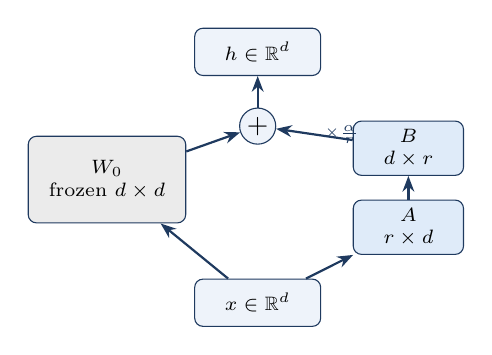
\begin{tikzpicture}[node distance=5mm]
        \node[box,minimum width=16mm] (x) {$x\in\mathbb{R}^{d}$};
        \node[box,above left=7mm and 1mm of x,minimum width=20mm,minimum height=11mm,fill=black!8] (W) {$W_0$\\\scriptsize frozen $d\times d$};
        \node[hot,above right=3mm and 4mm of x,minimum width=14mm] (A) {$A$\\\scriptsize $r\times d$};
        \node[hot,above=3mm of A,minimum width=14mm] (B) {$B$\\\scriptsize $d\times r$};
        \node[circle,draw=navy,fill=soft,inner sep=1pt,above=17mm of x] (plus) {$+$};
        \node[box,above=4mm of plus,minimum width=16mm] (h) {$h\in\mathbb{R}^{d}$};
        \draw[arr] (x) -- (W); \draw[arr] (x) -- (A); \draw[arr] (A) -- (B);
        \draw[arr] (W) -- (plus); \draw[arr] (B) -- node[right,font=\tiny]{$\times\frac{\alpha}{r}$} (plus);
        \draw[arr] (plus) -- (h);
      \end{tikzpicture}
      \vspace{1mm}

      {\small Frozen path in grey, trainable path in blue. $r\ll d$, e.g.\ $r=8$ and $d=768$.}
    \end{column}
  \end{columns}
\end{frame}

\begin{frame}{LoRA: the mathematics}
  \begin{columns}[T]
    \begin{column}{0.52\textwidth}
      \small
      \textbf{Forward pass}
      \[
        h = W_0x + \Delta W x = W_0x + \frac{\alpha}{r}\,B\,(A\,x)
      \]
      \begin{itemize}
        \item $A\in\mathbb{R}^{r\times d_{\text{in}}}$ compresses $x$ to $r$ numbers.
        \item $B\in\mathbb{R}^{d_{\text{out}}\times r}$ expands them back.
        \item $\alpha/r$ is a fixed \textbf{scaling factor}; $\alpha$ is a hyperparameter.
      \end{itemize}
      \textbf{Initialisation}: $A\sim\mathcal{N}(0,\sigma^2)$ (or Kaiming), and $B=0$.
      So $\Delta W=0$ at step 0, and the model starts \emph{exactly} as the pretrained one.
      \vspace{1mm}

      \textbf{Gradients}: $W_0$ gets none. Only $\frac{\partial\mathcal{L}}{\partial A}$ and $\frac{\partial\mathcal{L}}{\partial B}$ are computed and stored by the optimizer.
    \end{column}
    \begin{column}{0.44\textwidth}
      \begin{exampleblock}{Worked forward pass ($d=3$, $r=1$, $\alpha=1$)}
        \small
        $W_0=I$, $x=[2,1,0]^\top$, with $A$ and $B$ from the rank-1 slide.
        \[
          Ax=1\cdot2+0\cdot1+1\cdot0=2
        \]
        \[
          B(Ax)=[1,\,0,\,-1]^\top
        \]
        \[
          h=[2,1,0]^\top+[1,0,-1]^\top=[3,1,-1]^\top
        \]
        The correction costs $2dr=6$ multiplications, against $d^2=9$ for the frozen path.
      \end{exampleblock}
    \end{column}
  \end{columns}
\end{frame}

\begin{frame}{LoRA: counting parameters and memory for A1}
  \begin{columns}[T]
    \begin{column}{0.52\textwidth}
      \small
      LoRA on the query and value projections (\code{attn.q}, \code{attn.v}) of all 8 layers, with $r=8$:
      \[
        8\ \text{layers}\times2\ \text{matrices}\times(768\times8+8\times768)=196{,}608
      \]
      That is \textbf{0.24\%} of 82.1M.
      \vspace{2mm}

      \begin{tabular}{@{}lrr@{}}
        \toprule
        & Full FT & LoRA $r=8$\\
        \midrule
        Trainable params & 82.1M & 0.20M\\
        Adam state + grads & 985 MB & 2.4 MB\\
        Saved per task & 328 MB & 0.8 MB\\
        \bottomrule
      \end{tabular}
      \vspace{1mm}

      {\scriptsize fp32; the frozen weights (328 MB) are shared by all tasks. Activation memory is still needed for the backward pass.}
    \end{column}
    \begin{column}{0.44\textwidth}
      \begin{block}{Trainable fraction by target}
        \small
        With $r=8$ in A1, per layer:
        \begin{itemize}
          \item $q, v$: 24,576
          \item $q, k, v, o$: 49,152
          \item all linear layers (adds \code{fc} $768\to3072$ and \code{proj} $3072\to768$): 110,592
        \end{itemize}
        Over 8 layers that is 0.2M, 0.4M or 0.9M. All are tiny next to 82M.
      \end{block}
      \begin{exampleblock}{Note}
        \small
        The new task head, e.g.\ a $768\times13$ classifier for Phase 3, is always fully trained.
      \end{exampleblock}
    \end{column}
  \end{columns}
\end{frame}

\begin{frame}{LoRA: hyperparameters and where to apply it}
  \footnotesize
  \begin{tabularx}{\textwidth}{@{}l X X@{}}
    \toprule
    Knob & Meaning & Typical choice and effect\\
    \midrule
    Rank $r$ & number of directions of change & 4--64. Higher: more capacity, more overfitting risk\\
    Alpha $\alpha$ & strength of the update, via $\alpha/r$ & often $\alpha=2r$ or 16. With fixed $\alpha$, changing $r$ changes the step size\\
    Targets & which linear layers get $BA$ & $q,v$ is the original recipe. All linear layers usually work better at little cost\\
    LoRA dropout & dropout on $x$ before $A$ & 0.05--0.1 for small datasets such as NER folds\\
    Learning rate & for $A$ and $B$ only & about 10$\times$ the full fine-tuning rate, e.g.\ $2\times10^{-4}$ to $10^{-3}$\\
    Trainable extras & modules left unfrozen & the task head always, sometimes LayerNorms\\
    \bottomrule
  \end{tabularx}
  \vspace{2mm}
  \begin{exampleblock}{Mapping to our code}
    \small
    In our code LoRA would wrap \code{Attention.q/k/v/o}, \code{FeedForward.fc/proj} and \code{SwiGLU.gate/up/proj}. Embeddings and norms stay frozen.
  \end{exampleblock}
\end{frame}

\begin{frame}{LoRA: merging, task switching and inference}
  \begin{columns}[T]
    \begin{column}{0.5\textwidth}
      \small
      \textbf{Merging.} After training, fold the update into the weight once:
      \[
        W' = W_0 + \tfrac{\alpha}{r}BA
      \]
      The merged model has the \emph{original} shape and speed. There is \textbf{zero extra inference latency}.
      \vspace{2mm}

      \textbf{Un-merging.} $W_0 = W'-\tfrac{\alpha}{r}BA$ restores the base model.
      \vspace{1mm}

      \textbf{Task switching.} Keep one base model and one 0.8 MB adapter per task. Swap adapters in milliseconds.
    \end{column}
    \begin{column}{0.46\textwidth}
      \begin{exampleblock}{Capstone example}
        \small
        One A4 base model in GPU memory serves:
        \begin{itemize}
          \item the NER adapter (Phase 2);
          \item the rhetorical-role adapter (Phase 3);
          \item the judgment adapter (Phase 4); and so on.
        \end{itemize}
        The firm deploys \emph{one} model with small add-ons, not seven 330 MB models.
      \end{exampleblock}
      \begin{alertblock}{Careful}
        \small
        Measure latency \emph{after} merging. An unmerged adapter adds two small matrix products per wrapped layer.
      \end{alertblock}
    \end{column}
  \end{columns}
\end{frame}

\begin{frame}{LoRA: advantages, disadvantages and applications}
  \begin{columns}[T]
    \begin{column}{0.32\textwidth}
      \begin{exampleblock}{Advantages}
        \scriptsize
        \begin{itemize}
          \item 100--10,000$\times$ fewer trainable parameters.
          \item Much less optimizer memory, so larger batches fit on a T4.
          \item No inference latency after merging.
          \item Tiny per-task files; easy to swap.
          \item Starts exactly at the pretrained model ($B=0$), so training is stable.
          \item Less forgetting of pretrained knowledge.
          \item Often matches full fine-tuning.
        \end{itemize}
      \end{exampleblock}
    \end{column}
    \begin{column}{0.32\textwidth}
      \begin{alertblock}{Disadvantages}
        \scriptsize
        \begin{itemize}
          \item Low rank limits capacity. Tasks far from pretraining may need full fine-tuning.
          \item Extra hyperparameters: $r$, $\alpha$, targets.
          \item The same rank everywhere wastes budget (fixed by AdaLoRA).
          \item $\alpha/r$ scaling makes high ranks learn slowly (fixed by rsLoRA).
          \item Activation memory is unchanged; long sequences still cost.
          \item Merged adapters for several tasks cannot be batched together.
        \end{itemize}
      \end{alertblock}
    \end{column}
    \begin{column}{0.32\textwidth}
      \begin{block}{Applications}
        \scriptsize
        \begin{itemize}
          \item Instruction and domain tuning of large LLMs.
          \item Image-model styles, e.g.\ Stable Diffusion LoRAs.
          \item Serving many customers from one base model.
          \item \textbf{Capstone}: listed for Phases 2, 3 and 6, and the baseline every other family member is compared with. Examples: LoRA on $q,v$ plus a token head for NER; LoRA on all layers plus a sentence head for RR.
        \end{itemize}
      \end{block}
    \end{column}
  \end{columns}
\end{frame}

% ---------------------------------------------------------------- QLoRA
\begin{frame}{QLoRA: definition and intuition}
  \begin{columns}[T]
    \begin{column}{0.52\textwidth}
      \begin{block}{Definition (Dettmers et al., 2023)}
        \small
        \textbf{Quantised LoRA}: store the frozen base weights in \textbf{4-bit NormalFloat (NF4)}, and train ordinary LoRA adapters in 16-bit on top.
        Gradients flow \emph{through} the 4-bit weights into $A$ and $B$, but the 4-bit weights never change.
      \end{block}
      \footnotesize
      Three ingredients:
      \begin{enumerate}
        \item \textbf{NF4}: a 4-bit number format suited to normally distributed weights.
        \item \textbf{Double quantisation}: the scaling constants are quantised too.
        \item \textbf{Paged optimizers}: optimizer state spills to CPU RAM instead of crashing on memory spikes.
      \end{enumerate}
    \end{column}
    \begin{column}{0.44\textwidth}
      \begin{exampleblock}{Analogy}
        \small
        The statute book is photocopied at low resolution to fit in your bag. You can still read it clearly enough to write the amendment slips, and the slips themselves are written in full detail.
      \end{exampleblock}
      \begin{block}{Headline result}
        \small
        A 65B model was fine-tuned on one 48 GB GPU, matching 16-bit quality on the paper's benchmarks.
      \end{block}
    \end{column}
  \end{columns}
\end{frame}

\begin{frame}{QLoRA: NF4 quantisation}
  \begin{columns}[T]
    \begin{column}{0.5\textwidth}
      \small
      \textbf{Block-wise absmax quantisation}. Split $W$ into blocks of 64 weights. For each block:
      \[
        c=\max_i|w_i|,\qquad q_i=\operatorname*{arg\,min}_{v\in\text{NF4}}\Big|\frac{w_i}{c}-v\Big|
      \]
      Store the 4-bit index of $q_i$ and one constant $c$ per block.
      \textbf{Dequantise} when needed: $\hat w_i = c\cdot q_i$.
      \vspace{1mm}

      \textbf{NF4 levels}: 16 values in $[-1,1]$ at quantiles of $\mathcal N(0,1)$, including an exact 0. They are dense near 0, where most weights lie:
      \vspace{1mm}

      {\scriptsize $-1,\ -.70,\ -.53,\ -.39,\ -.28,\ -.18,\ -.09,\ 0,$\\
      $.08,\ .16,\ .25,\ .34,\ .44,\ .56,\ .72,\ 1$}
    \end{column}
    \begin{column}{0.46\textwidth}
      \begin{exampleblock}{Worked example (block of 4)}
        \small
        $w=[0.12,\,-0.40,\,0.05,\,0.33]$, so $c=0.40$.
        \[
          w/c=[0.30,\,-1.00,\,0.125,\,0.825]
        \]
        Nearest NF4 levels: $[0.34,\,-1,\,0.16,\,0.72]$.
        \[
          \hat w=[0.135,\,-0.40,\,0.064,\,0.289]
        \]
        The errors are at most 0.04, and each weight now needs 4 bits instead of 16.
      \end{exampleblock}
    \end{column}
  \end{columns}
\end{frame}

\begin{frame}{QLoRA: forward pass, double quantisation and paging}
  \begin{columns}[T]
    \begin{column}{0.5\textwidth}
      \small
      \textbf{Forward pass} (compute in bf16):
      \[
        h=\text{dequant}(W_0^{\text{NF4}})\,x+\tfrac{\alpha}{r}BAx
      \]
      \textbf{Backward pass}: gradients flow through the dequantised $W_0$ to reach $A$ and $B$. $W_0$ itself is never updated.
      \vspace{2mm}

      \textbf{Paged optimizers}: Adam states live in memory that can page to CPU RAM. A long document that briefly spikes memory slows down instead of crashing.
    \end{column}
    \begin{column}{0.46\textwidth}
      \begin{block}{Double quantisation}
        \small
        One fp32 constant per 64 weights adds $32/64=0.5$ bits per weight.
        Quantising the constants to 8 bits, in blocks of 256, cuts this to about $0.127$ bits.
      \end{block}
      \begin{exampleblock}{Memory for A1's frozen weights}
        \small
        \begin{tabular}{@{}lr@{}}
          fp32 & 328 MB\\
          fp16 / bf16 & 164 MB\\
          NF4 (+ constants) & $\approx$ 42 MB\\
        \end{tabular}
      \end{exampleblock}
    \end{column}
  \end{columns}
\end{frame}

\begin{frame}{QLoRA: advantages, disadvantages and applications}
  \begin{columns}[T]
    \begin{column}{0.32\textwidth}
      \begin{exampleblock}{Advantages}
        \scriptsize
        \begin{itemize}
          \item About 4$\times$ less memory for frozen weights than fp16, and 8$\times$ less than fp32.
          \item Fine-tunes models that would not otherwise fit on one GPU.
          \item Quality close to 16-bit LoRA in the paper.
          \item Same small adapter files as LoRA.
          \item Paged optimizers survive memory spikes from long documents.
        \end{itemize}
      \end{exampleblock}
    \end{column}
    \begin{column}{0.32\textwidth}
      \begin{alertblock}{Disadvantages}
        \scriptsize
        \begin{itemize}
          \item Slower per step: weights are dequantised on every forward and backward pass.
          \item Needs a CUDA GPU and the bitsandbytes kernels, not CPU or MPS.
          \item Quantisation error slightly perturbs the base model.
          \item Merging into 4-bit weights loses precision. You usually merge into a dequantised 16-bit copy.
          \item \textbf{Small gain for small models.} A1 in NF4 is about 41 MB instead of 164 MB (fp16), while activations dominate memory.
        \end{itemize}
      \end{alertblock}
    \end{column}
    \begin{column}{0.32\textwidth}
      \begin{block}{Applications}
        \scriptsize
        \begin{itemize}
          \item Fine-tuning 7B--70B LLMs on consumer or single data-centre GPUs.
          \item Low-budget academic research.
          \item \textbf{Capstone}: listed for Phases 3, 5, 6 and 7. Useful for your largest Phase-1 model (up to 300M), or a teacher model in distillation.
          \item Analyse the speed--memory--quality trade-off against 16-bit LoRA, since the memory saving at 80M is modest.
        \end{itemize}
      \end{block}
    \end{column}
  \end{columns}
\end{frame}

% ---------------------------------------------------------------- AdaLoRA
\begin{frame}{AdaLoRA: definition and intuition}
  \begin{columns}[T]
    \begin{column}{0.52\textwidth}
      \begin{block}{Definition (Zhang et al., 2023)}
        \small
        \textbf{Adaptive budget allocation for LoRA}. Instead of the same rank in every matrix, start with a generous rank everywhere.
        During training, measure how important each rank component is, and \emph{prune} the least important ones until a total budget is reached.
      \end{block}
      \begin{exampleblock}{Analogy}
        \small
        A chambers has 16 junior advocates to assign across 8 matters. At first everyone gets two. After a month, the complex matters get four and the routine ones get none.
      \end{exampleblock}
    \end{column}
    \begin{column}{0.44\textwidth}
      \begin{block}{Why it helps}
        \small
        Not all matrices matter equally. The paper found that the MLP layers and the \emph{top} layers usually need more rank than the bottom attention layers.
        A uniform rank wastes parameters where they are not needed and starves the layers that need them.
      \end{block}
      \begin{exampleblock}{Budget example}
        \small
        4 matrices start at rank 8 each (32 components). The target budget is 16.
        After pruning: top-layer $W_v$ has 7, top-layer MLP 5, bottom $W_v$ 3, bottom $W_q$ 1.
      \end{exampleblock}
    \end{column}
  \end{columns}
\end{frame}

\begin{frame}{AdaLoRA: the mathematics (1): SVD form and regulariser}
  \begin{columns}[T]
    \begin{column}{0.52\textwidth}
      \small
      \textbf{SVD-shaped update}
      \[
        \Delta W = P\,\Lambda\,Q
      \]
      with $P\in\mathbb{R}^{d\times r}$, $\Lambda=\operatorname{diag}(\lambda_1,\ldots,\lambda_r)$ and $Q\in\mathbb{R}^{r\times d}$.
      Component $i$ is the triplet $(P_{:,i},\lambda_i,Q_{i,:})$.
      \vspace{1mm}

      Removing component $i$ means setting $\lambda_i=0$. $P$ and $Q$ stay intact, so the component can come back later.
      \vspace{1mm}

      \textbf{Keep $P$ and $Q$ near-orthogonal}:
      \[
        R(P,Q)=\|P^\top P-I\|_F^2+\|QQ^\top-I\|_F^2
      \]
      \[
        \mathcal{L}_{\text{total}}=\mathcal{L}_{\text{task}}+\gamma\textstyle\sum_{\text{matrices}}R(P,Q)
      \]
    \end{column}
    \begin{column}{0.44\textwidth}
      \begin{exampleblock}{Why SVD form, not $BA$?}
        \small
        In $BA$, the rank directions are mixed together, so you cannot tell which one to delete.
        In $P\Lambda Q$ with orthogonal $P$ and $Q$, each $\lambda_i$ is the strength of one clean direction.
        Zeroing $\lambda_i$ removes exactly one direction, like dropping one singular value in an SVD.
      \end{exampleblock}
    \end{column}
  \end{columns}
\end{frame}

\begin{frame}{AdaLoRA: the mathematics (2): importance and budget}
  \begin{columns}[T]
    \begin{column}{0.52\textwidth}
      \small
      \textbf{Importance of a weight $w$} (sensitivity, smoothed over steps):
      \[
        s(w)=\big|\,w\cdot\tfrac{\partial\mathcal L}{\partial w}\big|,\quad
        \bar s_t=\beta_1\bar s_{t-1}+(1-\beta_1)s_t
      \]
      This estimates how much the loss would change if $w$ were removed.
      An uncertainty term discounts estimates that jump around.
      \vspace{1mm}

      \textbf{Score of component $i$}: the importance of $\lambda_i$, plus the average importance of $P$'s column $i$ and $Q$'s row $i$.
      \vspace{1mm}

      \textbf{Budget schedule}: the total rank $b(t)$ starts at about $1.5\times$ the target, is held during warm-up, then shrinks along a cubic curve to the target. At each step the lowest-scoring $\lambda_i$ are zeroed.
    \end{column}
    \begin{column}{0.44\textwidth}
      \begin{exampleblock}{Sensitivity example}
        \small
        Component 1: $\lambda_1=0.9$, gradient $0.5$, so $s=0.45$.\\
        Component 2: $\lambda_2=0.8$, gradient $0.01$, so $s=0.008$.
        \vspace{1mm}

        Changing component 2 barely changes the loss. It is pruned first, even though its $\lambda$ is large.
      \end{exampleblock}
    \end{column}
  \end{columns}
\end{frame}

\begin{frame}{AdaLoRA: advantages, disadvantages and applications}
  \begin{columns}[T]
    \begin{column}{0.32\textwidth}
      \begin{exampleblock}{Advantages}
        \scriptsize
        \begin{itemize}
          \item Better accuracy than LoRA at the same parameter budget, especially at small budgets.
          \item Removes the need to hand-tune rank per layer.
          \item The final rank pattern is \emph{interpretable}: it shows which layers the task needed.
          \item Pruned components can be revived during training.
          \item Merges into $W$ like LoRA, with no inference cost.
        \end{itemize}
      \end{exampleblock}
    \end{column}
    \begin{column}{0.32\textwidth}
      \begin{alertblock}{Disadvantages}
        \scriptsize
        \begin{itemize}
          \item More moving parts: budget schedule, warm-up, regulariser weight $\gamma$, smoothing $\beta$.
          \item Extra computation for importance scores and the orthogonality penalty; slower than LoRA.
          \item Importance estimates are noisy on small datasets.
          \item Needs a known number of training steps for the schedule.
          \item Harder to implement correctly by hand.
        \end{itemize}
      \end{alertblock}
    \end{column}
    \begin{column}{0.32\textwidth}
      \begin{block}{Applications}
        \scriptsize
        \begin{itemize}
          \item Tight parameter budgets, e.g.\ many tasks served on-device.
          \item Studying which layers a task relies on.
          \item \textbf{Capstone}: listed for Phases 3, 4, 5 and 6.
          \item Report the final rank map, e.g.\ ``CJPE put most rank in the top four MLP layers''. This is ready-made analysis for the report.
        \end{itemize}
      \end{block}
    \end{column}
  \end{columns}
\end{frame}

% ---------------------------------------------------------------- rsLoRA
\begin{frame}{rsLoRA: definition and the scaling problem}
  \begin{columns}[T]
    \begin{column}{0.52\textwidth}
      \begin{block}{Definition (Kalajdzievski, 2023)}
        \small
        \textbf{Rank-stabilised LoRA} is LoRA with one change: the scaling factor.
        \[
          \text{LoRA: } \gamma_r=\frac{\alpha}{r}\qquad\text{rsLoRA: } \gamma_r=\frac{\alpha}{\sqrt{r}}
        \]
      \end{block}
      \small
      \textbf{Why.} $BAx=\sum_{i=1}^{r} b_i\,(a_i^\top x)$ is a sum of $r$ roughly independent terms, so it grows like $\sqrt r$.
      \begin{itemize}
        \item $\times\frac1r$: the update shrinks like $\frac{1}{\sqrt r}$, so a large rank learns \emph{more slowly}.
        \item $\times\frac1{\sqrt r}$: the update stays the same size for any $r$.
      \end{itemize}
      The paper proves this keeps learning stable as $r$ grows.
    \end{column}
    \begin{column}{0.44\textwidth}
      \begin{exampleblock}{Numbers ($\alpha=16$)}
        \small
        \begin{tabular}{@{}rrr@{}}
          \toprule
          $r$ & $\alpha/r$ & $\alpha/\sqrt r$\\
          \midrule
          4 & 4.00 & 8.00\\
          16 & 1.00 & 4.00\\
          64 & 0.25 & 2.00\\
          256 & 0.0625 & 1.00\\
          \bottomrule
        \end{tabular}
        \vspace{1mm}

        With plain LoRA at $r=256$, the update is scaled down 64$\times$ compared with $r=4$. More rank then gives almost no benefit, which misleads rank experiments.
      \end{exampleblock}
    \end{column}
  \end{columns}
\end{frame}

\begin{frame}{rsLoRA: advantages, disadvantages and applications}
  \begin{columns}[T]
    \begin{column}{0.32\textwidth}
      \begin{exampleblock}{Advantages}
        \scriptsize
        \begin{itemize}
          \item A one-line change; no new parameters or cost.
          \item Higher ranks actually improve results, so a compute--quality trade-off becomes available.
          \item Learning rate transfers across ranks more reliably.
          \item Merges exactly like LoRA.
        \end{itemize}
      \end{exampleblock}
    \end{column}
    \begin{column}{0.32\textwidth}
      \begin{alertblock}{Disadvantages}
        \scriptsize
        \begin{itemize}
          \item No benefit at small ranks ($r\le8$), where it behaves like LoRA with a larger $\alpha$.
          \item High ranks cost more memory and time.
          \item Larger effective step sizes can destabilise training if the learning rate is not lowered.
          \item On its own it may look like a hyperparameter change. Argue clearly why it is a different method.
        \end{itemize}
      \end{alertblock}
    \end{column}
    \begin{column}{0.32\textwidth}
      \begin{block}{Applications}
        \scriptsize
        \begin{itemize}
          \item Whenever a task needs a large rank: complex domain shift, generation tasks.
          \item Fair rank-sweep studies.
          \item \textbf{Capstone}: listed for Phase 3. Natural for Phase 6 summarisation, which may need more capacity than classification.
          \item A clean experiment: LoRA and rsLoRA at $r\in\{8,32,128\}$, all else fixed. Does F1 keep rising with rank?
        \end{itemize}
      \end{block}
    \end{column}
  \end{columns}
\end{frame}

% ---------------------------------------------------------------- LORMA
\begin{frame}{LORMA: definition and intuition}
  \begin{columns}[T]
    \begin{column}{0.52\textwidth}
      \begin{block}{Definition (Bihany, Patel and Modi, 2025)}
        \small
        \textbf{Low-Rank Multiplicative Adaptation}. Instead of \emph{adding} a low-rank matrix to the frozen weight, LORMA \emph{multiplies} the frozen weight by a transformation built from low-rank factors:
        \[
          \text{LoRA: } W'=W_0+BA\qquad\text{LORMA: } W'=\mathcal{T}(BA)\,W_0
        \]
      \end{block}
      \begin{exampleblock}{Analogy}
        \small
        LoRA pastes an amendment slip \emph{next to} a section. LORMA applies a \emph{re-interpretation rule to} the section: ``read every mention of `court' as `tribunal'''.
        The original text is transformed, not supplemented.
      \end{exampleblock}
    \end{column}
    \begin{column}{0.44\textwidth}
      \begin{block}{Geometric view}
        \small
        A matrix multiplication can rotate and rescale.
        $\mathcal{T}(BA)\,W_0$ applies a learned rotation and scaling to the \emph{outputs} of $W_0$, reusing all the structure $W_0$ already has.
        An additive update instead has to express the change from scratch.
      \end{block}
      \begin{alertblock}{Compulsory in Phases 2--7}
        \small
        The course lists LORMA as compulsory in every adaptation phase. It comes from the course team's own paper, so expect viva questions on it.
      \end{alertblock}
    \end{column}
  \end{columns}
\end{frame}

\begin{frame}{LORMA: the mathematics (1): the rank problem}
  \begin{columns}[T]
    \begin{column}{0.52\textwidth}
      \small
      \textbf{The problem.} A naive multiplicative update $W'=(BA)\,W_0$ has
      \[
        \operatorname{rank}(BA\,W_0)\le r,
      \]
      so a full-rank $W_0$ would collapse to rank $r$, and the model would lose almost everything it knew.
      \vspace{1mm}

      \textbf{Rank inflation} fixes this. Two strategies are proposed:
      \begin{itemize}
        \item \textbf{Additive identity}: $W'=(I+BA)\,W_0$. With $B=0$ at the start, $W'=W_0$ exactly. The product stays full rank, and the low-rank part only \emph{adjusts} it.
        \item \textbf{Permutation-based}: rearrange the entries of $BA$ so the transform has a higher rank than $r$, without extra parameters.
      \end{itemize}
    \end{column}
    \begin{column}{0.44\textwidth}
      \begin{exampleblock}{Rank collapse, concretely}
        \small
        $d=768$ and $r=8$. $W_0$ has rank 768: it can produce outputs in 768 independent directions.
        $(BA)W_0$ can produce only 8. Every attention head would see nearly the same few directions.
        \vspace{1mm}

        With $(I+BA)W_0$ the identity keeps all 768 directions, and $BA$ tilts 8 of them.
      \end{exampleblock}
      \begin{alertblock}{Check the paper}
        \scriptsize
        This summarises the idea. Read the paper for the exact parameterisation, initialisation and scaling before implementing it.
      \end{alertblock}
    \end{column}
  \end{columns}
\end{frame}

\begin{frame}{LORMA: the mathematics (2): an efficient forward pass}
  \begin{columns}[T]
    \begin{column}{0.5\textwidth}
      \small
      Never form a $d\times d$ matrix. Compute the frozen output first, then correct it:
      \[
        h=(I+BA)W_0x = u + B(Au),\qquad u=W_0x
      \]
      \textbf{Extra cost}: $2dr$ multiplications per token, the same as LoRA.
      \vspace{1mm}

      \textbf{Difference from LoRA}: LoRA's correction reads the \emph{input} $x$. LORMA's reads the \emph{output} $u=W_0x$, the already-processed signal.
      \vspace{1mm}

      \textbf{Merging}: compute $W'=(I+BA)W_0$ once after training, so inference costs nothing extra.
    \end{column}
    \begin{column}{0.46\textwidth}
      \begin{exampleblock}{Worked example ($d=3$, $r=1$)}
        \small
        $u=W_0x=[2,1,0]^\top$, $A=[1,0,1]$, $B=[0.5,0,-0.5]^\top$.
        \[
          Au=2,\quad B(Au)=[1,0,-1]^\top
        \]
        \[
          h=u+B(Au)=[3,1,-1]^\top
        \]
        This equals the LoRA example only because $W_0=I$ there. For any other $W_0$ the two methods give different outputs.
      \end{exampleblock}
    \end{column}
  \end{columns}
\end{frame}

\begin{frame}{LORMA: advantages, disadvantages and applications}
  \begin{columns}[T]
    \begin{column}{0.32\textwidth}
      \begin{exampleblock}{Advantages}
        \scriptsize
        \begin{itemize}
          \item Same number of trainable parameters as LoRA at the same $r$.
          \item Reuses the structure of $W_0$ by transforming it, a different inductive bias.
          \item The paper reports competitive or better results than LoRA, and faster convergence in some settings.
          \item Mergeable: $W'=(I+BA)W_0$ can be computed once, so there is no inference cost.
          \item Starts exactly at the pretrained model when $B=0$.
        \end{itemize}
      \end{exampleblock}
    \end{column}
    \begin{column}{0.32\textwidth}
      \begin{alertblock}{Disadvantages}
        \scriptsize
        \begin{itemize}
          \item Needs rank inflation. Without it, the model collapses.
          \item Unmerged training costs an extra pass through $W_0$'s outputs, $B(A(W_0x))$.
          \item Gradients for $A$ and $B$ depend on $W_0$, so scaling and learning rate may need retuning relative to LoRA.
          \item Less tooling: mainstream PEFT libraries do not provide it, so you must implement it yourself.
          \item Fewer independent results than LoRA.
        \end{itemize}
      \end{alertblock}
    \end{column}
    \begin{column}{0.32\textwidth}
      \begin{block}{Applications}
        \scriptsize
        \begin{itemize}
          \item Parameter-efficient adaptation wherever LoRA is used.
          \item \textbf{Capstone}: \alert{compulsory} in Phases 2--7, and on all four Phase-1 architectures.
          \item Best report experiment: LoRA vs LORMA at identical $r$, targets and budget, on each architecture.
          \item Compare convergence speed (loss vs step), not only final F1.
        \end{itemize}
      \end{block}
    \end{column}
  \end{columns}
\end{frame}

% ---------------------------------------------------------------- summary
\begin{frame}{The LoRA family side by side}
  \footnotesize
  \begin{tabularx}{\textwidth}{@{}l>{\raggedright\arraybackslash}p{3.3cm}>{\raggedright\arraybackslash}X>{\raggedright\arraybackslash}X>{\raggedright\arraybackslash}X@{}}
    \toprule
    Method & Update & Trainable params & Main benefit & Main cost\\
    \midrule
    LoRA & $W_0+\frac{\alpha}{r}BA$ & $2dr$ per matrix & simple, mergeable, strong default & fixed rank; weak scaling at high $r$\\
    QLoRA & $\text{deq}(W_0^{\text{NF4}})+\frac{\alpha}{r}BA$ & same as LoRA & 4-bit frozen weights; big models fit & slower; CUDA only; small gain at 80M\\
    AdaLoRA & $W_0+P\Lambda Q$, pruned & starts $\approx1.5\times$ budget, ends at budget & rank goes where needed & complex schedule; slower\\
    rsLoRA & $W_0+\frac{\alpha}{\sqrt r}BA$ & same as LoRA & high ranks keep learning & needs a larger $r$ to matter\\
    LORMA & $(I+BA)\,W_0$ & same as LoRA & multiplicative; reuses $W_0$ & rank inflation; self-implemented\\
    \bottomrule
  \end{tabularx}
  \vspace{2mm}
  \begin{exampleblock}{Choosing quickly}
    \small
    Start with LoRA. Use rsLoRA if raising $r$ stops helping. Use AdaLoRA when parameters are scarce or you want a layer-importance map. Use QLoRA when memory, not quality, is the limit. Use LORMA always, since it is required, and compare it against LoRA at matched settings.
  \end{exampleblock}
\end{frame}

\begin{frame}{Using the LoRA family in Phases 2--7}
  \begin{columns}[T]
    \begin{column}{0.5\textwidth}
      \small
      \textbf{A recipe that satisfies the rules}
      \begin{enumerate}
        \item Load each Phase-1 model (A1--A4) and freeze it.
        \item Add the task head (token, sentence or document).
        \item Wrap the chosen linear layers with LoRA, LORMA, AdaLoRA, and so on.
        \item Train the head and adapters only.
        \item Log trainable parameters, memory, time and the task metric.
        \item Merge, then measure inference speed.
      \end{enumerate}
      Each method is a \textbf{different technique}. Changing only $r$ or $\alpha$ is a hyperparameter change and does not count.
    \end{column}
    \begin{column}{0.46\textwidth}
      \begin{block}{A fair comparison table for the report}
        \scriptsize
        \begin{tabular}{@{}lrrr@{}}
          \toprule
          Method & Trainable & Memory & Macro-F1\\
          \midrule
          Full FT & 82.1M & \ldots & \ldots\\
          LoRA $r=8$ & 0.20M & \ldots & \ldots\\
          rsLoRA $r=64$ & 1.57M & \ldots & \ldots\\
          AdaLoRA $b=8$ & 0.20M & \ldots & \ldots\\
          LORMA $r=8$ & 0.20M & \ldots & \ldots\\
          \bottomrule
        \end{tabular}
        \vspace{1mm}

        Fill in from your runs, with identical data, head and epochs.
      \end{block}
      \begin{alertblock}{Pitfalls}
        \scriptsize
        Forgetting $B=0$; too low a learning rate; ignoring the $\alpha/r$ effect when changing $r$.
      \end{alertblock}
    \end{column}
  \end{columns}
\end{frame}

% =====================================================================
\section{Evaluation metrics}

\begin{frame}{Precision, recall and F1}
  \begin{columns}[T]
    \begin{column}{0.5\textwidth}
      \small
      \[ P=\frac{\text{correct predictions}}{\text{all predictions}} \]
      \[ R=\frac{\text{correct predictions}}{\text{all gold items}} \]
      \[
        F_1=\frac{2PR}{P+R}\quad\text{(harmonic mean)}
      \]
      \textbf{Precision} asks: of what I said, how much was right?
      \textbf{Recall} asks: of what was there, how much did I find?
    \end{column}
    \begin{column}{0.46\textwidth}
      \begin{exampleblock}{Example (NER)}
        \small
        The document has 14 gold entities. The model predicts 10, and 7 of them are exactly right.
        \[
          P=\tfrac{7}{10}=0.70,\quad R=\tfrac{7}{14}=0.50
        \]
        \[
          F_1=\tfrac{2(0.70)(0.50)}{1.20}=0.583
        \]
        The harmonic mean punishes imbalance. $P=1$ with $R=0.01$ gives $F_1\approx0.02$, not 0.5.
      \end{exampleblock}
    \end{column}
  \end{columns}
\end{frame}

\begin{frame}{Macro, micro and subset accuracy}
  \twoterms{Macro-F1 vs Micro-F1}
  {\textbf{Macro}: compute F1 per class, then average the classes equally. \textbf{Micro}: pool all decisions first, then compute one F1. Macro rewards rare classes.}
  {The class ``Fact'' has 900 sentences with F1 0.90. ``Dissent'' has 10 with F1 0.30. Macro-F1 is $(0.90+0.30)/2=0.60$. Micro-F1 stays near 0.89, because ``Fact'' dominates the pooled counts.}
  {Subset accuracy and Micro-F1@7}
  {\textbf{Subset accuracy}: a multi-label prediction counts only if the whole set is exactly right. \textbf{@7}: only the top 7 retrieved items are scored.}
  {Gold $\{302,120B\}$, predicted $\{302\}$: subset accuracy is 0, though partly right. Retrieval: 5 relevant cases, 3 of them in the top 7, so $P@7=3/7=0.43$ and $R@7=3/5=0.60$.}
\end{frame}

\begin{frame}{Class imbalance}
  \term{Class imbalance}
  {Some labels are far more frequent than others. A model can score well on accuracy by always predicting the common class, yet be useless for the rare ones. Fixes include class weights, resampling, and tuned thresholds.}
  {In CJPE, suppose 80\% of appeals are dismissed. ``Always predict dismissed'' gets 80\% accuracy. Its Macro-F1 is only about 0.44, because recall on ``allowed'' is 0. A class weight of 4 on ``allowed'' makes each of those mistakes cost four times as much.}
\end{frame}

\begin{frame}{BERTScore (Phase 1 and Phase 6 primary metric)}
  \begin{columns}[T]
    \begin{column}{0.5\textwidth}
      \small
      \begin{enumerate}
        \item A pretrained encoder turns every token of the reference $r$ and the hypothesis $h$ into a \textbf{contextual embedding}: a vector whose value depends on the surrounding words.
        \item Each token is matched to its most similar token on the other side, by \textbf{cosine similarity}.
        \item These matches give recall, precision and F1:
      \end{enumerate}
      \[ R=\tfrac1{|r|}\textstyle\sum_{i}\max_j\cos(\mathbf r_i,\mathbf h_j) \]
      \[ P=\tfrac1{|h|}\textstyle\sum_{j}\max_i\cos(\mathbf r_i,\mathbf h_j),\quad F_1=\tfrac{2PR}{P+R} \]
    \end{column}
    \begin{column}{0.46\textwidth}
      \begin{exampleblock}{Example}
        \small
        Reference: ``the petition was rejected''.\\
        Hypothesis: ``the appeal was dismissed''.
        \vspace{1mm}

        Exact-word metrics see only ``the'' and ``was'' in common.
        BERTScore finds that \emph{dismissed} and \emph{rejected}, and \emph{appeal} and \emph{petition}, have similar embeddings.
        It gives a high score for the right \emph{meaning}.
      \end{exampleblock}
      \begin{block}{Cosine similarity}
        \small
        $\cos(\mathbf a,\mathbf b)=\frac{\mathbf a\cdot\mathbf b}{\|\mathbf a\|\|\mathbf b\|}$: 1 means the same direction and 0 means unrelated. Example: $\cos([1,0],[1,1])=1/\sqrt2\approx0.71$.
      \end{block}
    \end{column}
  \end{columns}
\end{frame}

\begin{frame}{ROUGE-L and BLEU-4}
  \twoterms{ROUGE-L (longest common subsequence)}
  {Find the longest sequence of words that appears in both texts in the same order, though not necessarily adjacent. Precision and recall are its length over each text's length.}
  {Ref: ``the appeal is dismissed with costs''. Hyp: ``the appeal is allowed with costs''. The LCS is ``the appeal is with costs'', 5 words. So $P=R=5/6$ and ROUGE-L $=0.83$, even though the \emph{meaning} is reversed.}
  {BLEU-4}
  {The geometric mean of 1-, 2-, 3- and 4-gram precisions, times a \textbf{brevity penalty} $\text{BP}=e^{1-|r|/|h|}$ when the hypothesis is shorter than the reference.}
  {In the same pair, none of the 3 hypothesis 4-grams (``the appeal is allowed'', \ldots) appears in the reference. Unsmoothed BLEU-4 is therefore 0, though 5 of 6 words match. A hypothesis half the reference length gets $\text{BP}=e^{-1}=0.37$.}
\end{frame}

\begin{frame}{Perplexity vs generation metrics, and bits per word}
  \twoterms{Why loss is not the whole story}
  {Validation loss measures how well the model predicts the \emph{true} next token. BERTScore measures what the model \emph{actually writes} after a decoding choice. The two can disagree.}
  {Two models have loss 2.40 and 2.45. With temperature 1.2 the better one rambles; with temperature 0.7 the worse one writes tight legal prose. The decoding choice decides the BERTScore ranking.}
  {Bits per word}
  {Total loss over a text, in bits, divided by its number of \emph{words}. Unlike per-token loss, it is comparable across tokenizers.}
  {Tokenizer A: 1.3 tokens/word at 2.0 nats/token, so $1.3\times2.0/\ln2=3.75$ bits/word. Tokenizer B: 1.1 tokens/word at 2.3 nats/token, so 3.65 bits/word. B is better, though its per-token loss looks worse.}
\end{frame}

% =====================================================================
\section{Data engineering}

\begin{frame}{Tokens, corpus and budget}
  \twoterms{Token and corpus}
  {A \textbf{token} is the unit a model reads: a word, a piece of a word, or a symbol. A \textbf{corpus} is the collection of training text.}
  {``appellant's'' may become three tokens: \code{appell}, \code{ant} and \code{'s}. The Phase-1 corpus has more than 4.5 billion tokens across four sources.}
  {Token budget and data mixing}
  {The \textbf{budget} is how many tokens you choose to train on. \textbf{Mixing ratios} set each source's share of it.}
  {A 200M budget with Acts at 0.10 means 20M tokens of statutes. Setting Acts to 0 is an \emph{ablation}: does the model's judgment writing improve or suffer without them?}
\end{frame}

\begin{frame}{File formats and streaming}
  \twoterms{JSON and JSON Lines}
  {\textbf{JSON} stores nested data as one document. \textbf{JSON Lines} (JSONL) stores one complete JSON object per line.}
  {JSON: \code{[\{"text":"A"\},\{"text":"B"\}]}. JSONL has the same data on two lines: \code{\{"text":"A"\}} then \code{\{"text":"B"\}}. JSONL can be read line by line; a JSON array needs a streaming parser.}
  {Streaming (ijson)}
  {Read a file record by record, keeping only the current record in memory. The whole file is never loaded.}
  {The 10.7 GB High Courts file would not fit in a 12 GB Colab RAM with Python overhead. Streaming reads one judgment, writes it out, and discards it, using a few megabytes.}
\end{frame}

\begin{frame}{Splitting without cheating}
  \twoterms{Data leakage}
  {Validation or test information reaching the model during training. It makes scores look better than they will be on truly new data.}
  {One judgment is cut into 1,024-token blocks. Block 3 goes to training and block 4 to validation. The model has already seen the case facts, so validation loss is too optimistic.}
  {Document-level split}
  {Assign whole documents to train or validation, never both. We use this.}
  {Judgment \#881 goes entirely to validation. Its prompts in the dev set are therefore genuinely unseen, just as the hidden test prompts are.}
\end{frame}

\begin{frame}{Storage for fast training}
  \twoterms{Token bin and uint16}
  {All token IDs are written into one flat binary file. \code{uint16} is an unsigned 16-bit integer (0 to 65,535), so each token takes 2 bytes.}
  {200M tokens take 400 MB as uint16, and 1.6 GB as Python's default 64-bit integers. A 32k vocabulary fits under 65,535, so uint16 is enough.}
  {Memory map (memmap)}
  {Treat a file on disk as if it were an array in memory. The operating system loads only the pages you touch.}
  {Training asks for tokens 5,000,000 to 5,001,025. Only those 2 KB are read from disk, not the whole 400 MB file.}
\end{frame}

\begin{frame}{Special tokens and dev-set construction}
  \twoterms{End-of-text token}
  {A special token, \code{<|endoftext|>}, placed between documents. It tells the model that one text ends here and another begins.}
  {``\ldots appeal dismissed. \code{<|endoftext|>} IN THE HIGH COURT OF DELHI \ldots''. The model learns not to carry names from one case into the next. During Phase-1 generation we \emph{ban} it, so the model never stops early.}
  {Dev set}
  {Our own labelled stand-in for the hidden test set. It has the same format, built from held-out documents.}
  {Take held-out judgment \#881, choose a random 640-word window, and use the first 512 words as the prompt. The next 128 words become the reference answer.}
\end{frame}

% =====================================================================
\section{Tokenization}

\begin{frame}{Tokenizer and vocabulary}
  \twoterms{Tokenizer}
  {Converts text to a list of integer IDs, and back again. The model only ever sees the integers.}
  {``The appellant'' becomes \code{[412, 2871]} and then decodes back to ``The appellant''. Every other stage works on those numbers.}
  {Vocabulary and special tokens}
  {The fixed set of tokens the tokenizer knows. Its size $V$ sets the width of the embedding table and the output layer.}
  {With $V=32{,}000$, token 2871 might be ``Ġappellant'' (Ġ marks a leading space). A larger vocabulary means shorter sequences but more embedding parameters.}
\end{frame}

\begin{frame}{Byte-Pair Encoding (BPE), step by step}
  \begin{columns}[T]
    \begin{column}{0.52\textwidth}
      \small
      \textbf{Idea:} start from single characters (or bytes). Repeatedly merge the \emph{most frequent adjacent pair} into a new token until the vocabulary reaches its target size.
      \vspace{2mm}

      Toy corpus word counts: \emph{appeal} $\times10$, \emph{appellant} $\times8$, \emph{apply} $\times5$.
      \vspace{1mm}

      \begin{tabular}{@{}lll@{}}
        \toprule
        Merge & Pair (count) & New token\\
        \midrule
        1 & a + p (23) & \code{ap}\\
        2 & ap + p (23) & \code{app}\\
        3 & app + e (18) & \code{appe}\\
        4 & appe + l (18) & \code{appel}\\
        $\ldots$ & & \code{appeal}, \code{appell}\\
        \bottomrule
      \end{tabular}
    \end{column}
    \begin{column}{0.44\textwidth}
      \begin{exampleblock}{Why this works}
        \small
        Frequent words become \textbf{one token}. Rare words are split into known pieces:
        \vspace{1mm}

        \emph{appellant} $\to$ \code{appell} + \code{ant}\\
        \emph{appellate} $\to$ \code{appell} + \code{ate}
        \vspace{1mm}

        The model can reuse what it learned about \code{appell}. No word is ever ``unknown''.
      \end{exampleblock}
    \end{column}
  \end{columns}
\end{frame}

\begin{frame}{Byte-level BPE and the unknown-token problem}
  \twoterms{Byte-level BPE}
  {BPE that starts from the 256 possible bytes instead of characters. Any text can be encoded, because every string is a sequence of bytes.}
  {A judgment quoting the Devanagari name ``\,\textit{Ram}\,'', or the symbol ``\S'', is split into its UTF-8 bytes and still encoded. Nothing is lost.}
  {Unknown token (unk) and OOV}
  {Word-level tokenizers map words outside their vocabulary (\emph{out-of-vocabulary}) to a single \code{<unk>} token. Byte-level BPE never needs it.}
  {A word-level tokenizer trained on news would turn ``Vakalatnama'' into \code{<unk>}, and the model could never write it. Our legal BPE learns it, or splits it into pieces.}
\end{frame}

\begin{frame}{Fertility and GPT-2's tokenizer}
  \twoterms{Fertility (tokens per word)}
  {The average number of tokens per word. Lower fertility means shorter sequences: more text fits in the context window, and each training step covers more words.}
  {A prompt has 512 words. At fertility 1.35 it is about 690 tokens, which fits in 1,024 with room for the answer. At fertility 1.8 it is 920 tokens, leaving only 104 for the continuation.}
  {GPT-2 tokenizer}
  {A 50,257-token byte-level BPE trained on web text. The starter notebook uses it. It is allowed, because it is a tokenizer and not pretrained model weights.}
  {The web is full of ``Ġthe'' and ``Ġemail''. Legal words like ``respondent'' may cost 2 to 3 GPT-2 tokens but only 1 in a legal BPE. That is exactly what \code{--compare-gpt2} measures.}
\end{frame}

% =====================================================================
\section{Language modelling basics}

\begin{frame}{What a language model does}
  \twoterms{Language model (LM)}
  {A model that assigns probabilities to text. Equivalently, it gives a probability for the next token, given the tokens so far.}
  {After ``The appeal is hereby'', a good legal LM gives ``dismissed'' 0.45, ``allowed'' 0.30, ``disposed'' 0.15, and ``banana'' nearly 0.}
  {Autoregressive / causal LM}
  {Generates one token at a time. Each new token is appended to the input, and the model predicts again. ``Causal'' means each position may use only the past.}
  {``The'' $\to$ ``appeal'' $\to$ ``is'' $\to$ ``dismissed'': four passes, each feeding on the previous output. This is how the 128-word continuation is written.}
\end{frame}

\begin{frame}{Logits and softmax}
  \begin{columns}[T]
    \begin{column}{0.5\textwidth}
      \term{Logits}
      {The raw, unnormalised scores the model outputs, one per vocabulary token. Higher means more likely. They can be negative.}
      {For the next word after ``The appeal is'': dismissed $2.0$, allowed $1.0$, pending $0.0$.}
    \end{column}
    \begin{column}{0.46\textwidth}
      \term{Softmax}
      {Turns logits $z$ into probabilities that are positive and sum to 1: $p_i=e^{z_i}/\sum_j e^{z_j}$.}
      {$e^{2}=7.39$, $e^{1}=2.72$, $e^{0}=1$, and the sum is $11.11$. So $p=[0.665,\,0.245,\,0.090]$ for dismissed, allowed and pending.}
    \end{column}
  \end{columns}
\end{frame}

\begin{frame}{Cross-entropy loss and perplexity}
  \twoterms{Cross-entropy loss}
  {The negative log-probability the model gave the \emph{correct} token, averaged over positions: $\mathcal{L}=-\frac1T\sum_t\log p(x_t\mid x_{<t})$. Lower is better.}
  {If the true word is ``dismissed'' ($p=0.665$), the loss is $-\ln 0.665 = 0.41$. If it was ``pending'' ($p=0.09$), the loss is $-\ln0.09=2.41$. Confident wrong guesses cost the most.}
  {Perplexity (PPL)}
  {$e^{\mathcal{L}}$: the effective number of equally likely choices the model is ``torn between'' at each step.}
  {Loss 3.0 gives PPL $e^3\approx20$: like choosing among 20 words each time. Loss 2.3 gives about 10. A uniform guess over 32,000 tokens has PPL 32,000.}
\end{frame}

\begin{frame}{Context, prefix and continuation loss}
  \twoterms{Context window (block size)}
  {The maximum number of tokens the model reads at once. Ours is 1,024.}
  {The 690-token prompt plus about 180 generated tokens is 870, which fits in 1,024. A 3,000-token judgment does not fit, and must be truncated or chunked.}
  {Prefix and continuation loss}
  {The \textbf{prefix} is the given context; the model is scored only on the tokens after it. With a prefix of $p$ tokens, loss is averaged over positions $p+1,\ldots,T$.}
  {With $p=768$ in a 1,025-token block, the model reads 768 tokens and is scored on the next 257. This mirrors Phase 1 exactly: read the prompt, then write.}
\end{frame}

\begin{frame}{Parameters and what ``from scratch'' means}
  \twoterms{Parameters (weights)}
  {The learned numbers inside the model. \textbf{Embedding} parameters are the token table. \textbf{Non-embedding} parameters are everything else.}
  {A1 has 82.1M parameters: 24.6M in the $32{,}064\times768$ embedding table and 57.5M elsewhere (the blocks plus the position table). The rules require 50M to 300M.}
  {From scratch vs pretrained}
  {\textbf{From scratch}: weights start random, and all knowledge comes from our training. \textbf{Pretrained}: weights downloaded from a model someone else trained. That is forbidden here.}
  {Before training, our model writes ``appeal xyl the the Qz''. After 200M tokens of legal text it writes ``appeal is dismissed with costs''. Every bit of that came from the provided corpus.}
\end{frame}

% =====================================================================
\section{Transformer building blocks}

\begin{frame}{Embeddings}
  \twoterms{Token embedding}
  {A lookup table that maps each token ID to a learned vector of $d$ numbers. Tokens with similar meaning end up with similar vectors.}
  {Token 2871 (``appellant'') maps to row 2871 of a $32{,}000\times768$ table, a 768-number vector. After training, ``appellant'' and ``petitioner'' sit close together.}
  {Tied embeddings}
  {The output layer that scores the next token reuses the input embedding table, instead of learning a separate one.}
  {This saves $32{,}064\times768 = 24.6$M parameters. It also makes sense: if ``appellant'' \emph{means} vector $v$, the model should predict it when its hidden state looks like $v$.}
\end{frame}

\begin{frame}{Self-attention: queries, keys and values}
  \begin{columns}[T]
    \begin{column}{0.52\textwidth}
      \small
      Each token makes three vectors from its embedding:
      \begin{itemize}
        \item \textbf{Query $q$}: what am I looking for?
        \item \textbf{Key $k$}: what do I contain?
        \item \textbf{Value $v$}: what do I pass on if chosen?
      \end{itemize}
      \[
        \text{Attention}(Q,K,V)=\text{softmax}\!\Big(\frac{QK^\top}{\sqrt{d_h}}\Big)V
      \]
      Each output is a weighted average of the values. The weights come from query--key similarity.
      Dividing by $\sqrt{d_h}$ keeps scores from growing with the vector size.
    \end{column}
    \begin{column}{0.44\textwidth}
      \begin{exampleblock}{Example}
        \small
        ``The \textbf{respondent} filed a reply, but \textbf{he} did not appear.''
        \vspace{1mm}

        The query of ``he'' matches the key of ``respondent'' strongly, with a score of 0.8.
        So ``he'' mostly copies the value of ``respondent'', and the model now ``knows'' who ``he'' is.
        \vspace{1mm}

        Numerically: $q\cdot k = 16$ with $d_h=64$ gives $16/8=2.0$ before the softmax.
      \end{exampleblock}
    \end{column}
  \end{columns}
\end{frame}

\begin{frame}{Multi-head attention and head dimension}
  \term{Multi-head attention (MHA)}
  {Run several attention operations (\emph{heads}) in parallel, each on a slice of the vector of size $d_h=d/H$, and concatenate their outputs. Different heads learn different relationships.}
  {With $d=768$ and $H=12$ heads, each head works on $d_h=64$ numbers. In a judgment, one head might link pronouns to parties (``he'' $\to$ ``respondent''). Another might link ``Section'' to its number (``302''). A third might track the case citation being discussed.}
\end{frame}

\begin{frame}{Attention masks}
  \begin{columns}[T]
    \begin{column}{0.56\textwidth}
      \small
      A \textbf{mask} decides which keys each query may see. Blocked scores are set to $-\infty$, so their softmax weight is 0.
      \vspace{1mm}
      \begin{itemize}
        \item \textbf{Causal}: see only the past. This is needed for generation, or the model could peek at the answer.
        \item \textbf{Bidirectional}: see everything. Good for \emph{reading} a prompt.
        \item \textbf{Prefix}: bidirectional inside the prompt, causal after it.
        \item \textbf{Sliding window}: see only the last $W$ tokens.
      \end{itemize}
      \textcolor{exgreen}{\textbf{Example.}} When predicting word 5, a causal mask stops the model from seeing word 5 itself. Without it, training would be trivial copying.
    \end{column}
    \begin{column}{0.4\textwidth}
      \centering
      \maskgrid{causal}{\j<=\i ? 1 : 0}\hspace{2mm}
      \maskgrid{bidirectional}{1}\\[2mm]
      \maskgrid{prefix, $p=3$}{(\j<3 || \j<=\i) ? 1 : 0}\hspace{2mm}
      \maskgrid{window $W=2$}{(\j<=\i && \j>\i-2) ? 1 : 0}\\[1mm]
      {\scriptsize rows = queries, columns = keys}
    \end{column}
  \end{columns}
\end{frame}

\begin{frame}{Residual connections and normalisation}
  \twoterms{Residual connection}
  {Add a layer's input to its output: $x\leftarrow x+f(x)$. The layer only has to learn a \emph{correction}, and gradients flow straight through deep stacks.}
  {Like editing a draft with tracked changes rather than rewriting it from scratch each round. If a layer has nothing useful to add, $f(x)\approx0$ and the draft passes through unchanged.}
  {LayerNorm and pre-LN}
  {LayerNorm rescales each vector to mean 0 and variance 1, then applies a learned scale and shift. \textbf{Pre-LN} normalises \emph{before} each sub-layer, which trains more stably.}
  {$x=[2,4,6]$ has mean 4 and standard deviation 1.63, giving $[-1.22,\,0,\,1.22]$. The numbers keep their shape, but no layer can blow them up to $[2000,4000,6000]$.}
\end{frame}

\begin{frame}{RMSNorm and the feed-forward network}
  \twoterms{RMSNorm}
  {Divide by the root-mean-square only; there is no mean subtraction and no bias: $x/\sqrt{\frac1d\sum x_i^2+\epsilon}\odot g$. It is cheaper and works as well in practice.}
  {$x=[2,4,6]$: $\text{rms}=\sqrt{(4+16+36)/3}=4.32$, giving $[0.46,\,0.93,\,1.39]$. Compare LayerNorm's $[-1.22,0,1.22]$: the shape is similar, with less arithmetic.}
  {MLP / feed-forward network (FFN)}
  {After attention mixes information \emph{between} tokens, a two-layer network processes each token \emph{on its own}: expand to $4d$, apply a non-linearity, project back to $d$.}
  {Attention gathers ``he = respondent''. The MLP then works with that fact, for example ``a respondent who did not appear suggests an \emph{ex parte} order''. Roughly two thirds of a block's parameters live here.}
\end{frame}

\begin{frame}{Activation functions}
  \begin{columns}[T]
    \begin{column}{0.5\textwidth}
      \small
      \begin{itemize}
        \item \textbf{ReLU}: $\max(0,x)$. $\text{ReLU}(-2)=0$, $\text{ReLU}(3)=3$. Simple, but ``dead'' for negatives.
        \item \textbf{GELU}: $x\cdot\Phi(x)$, a smooth ReLU. $\text{GELU}(-0.5)\approx-0.15$, so small negatives leak through.
        \item \textbf{SiLU}: $x\cdot\sigma(x)$. $\text{SiLU}(1)=0.73$.
        \item \textbf{SwiGLU}: $W_2\big(\text{SiLU}(W_gx)\odot W_ux\big)$. One branch computes content; the other acts as a learned \emph{gate} that says how much of it passes.
      \end{itemize}
    \end{column}
    \begin{column}{0.46\textwidth}
      \centering
      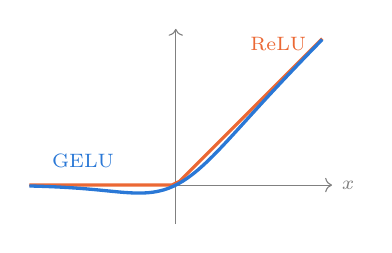
\begin{tikzpicture}[scale=0.62]
        \draw[->,gray] (-3,0)--(3.2,0) node[right,font=\scriptsize]{$x$};
        \draw[->,gray] (0,-0.8)--(0,3.2);
        \draw[very thick,warm,domain=-3:3,samples=40] plot (\x,{max(0,\x)});
        \draw[very thick,accent,domain=-3:3,samples=60] plot (\x,{\x/(1+exp(-1.702*\x))});
        \node[font=\scriptsize,warm] at (2.1,2.9) {ReLU};
        \node[font=\scriptsize,accent] at (-1.9,0.5) {GELU};
      \end{tikzpicture}
      \begin{exampleblock}{SwiGLU as a valve}
        \small
        Content says ``this token is a date''. The gate says ``0.1: dates matter little here''. The output is a mostly closed valve.
      \end{exampleblock}
    \end{column}
  \end{columns}
\end{frame}

\begin{frame}{Dropout and weight initialisation}
  \twoterms{Dropout}
  {During training, randomly zero a fraction $p$ of activations, so the network cannot rely on any single unit. It is turned off at inference.}
  {With $p=0.1$, one in ten features is hidden at each step. It is like studying with random lines of your notes covered, so you must understand the case and not memorise one line. With 200M tokens and one pass, overfitting is rare, so we default to 0.}
  {Weight initialisation}
  {The random starting values. We draw from $\mathcal{N}(0,0.02^2)$ and shrink residual output layers by $1/\sqrt{2L}$ so the sum of $L$ layers does not explode.}
  {With 8 layers, the output projections start with standard deviation $0.02/\sqrt{16}=0.005$. Adding 16 residual updates then keeps the signal near its starting size.}
\end{frame}

% =====================================================================
\section{Architectures}

\begin{frame}{Encoder, decoder and cross-attention}
  \twoterms{Encoder vs decoder}
  {An \textbf{encoder} reads a whole input with bidirectional attention and produces vectors. A \textbf{decoder} generates text causally, one token at a time.}
  {An encoder is the judge reading the full case file, where every page may refer to every other. A decoder is the judge writing the order, word by word, unable to see words not yet written.}
  {Cross-attention}
  {Decoder queries attend to the \emph{encoder's} keys and values. This is how the writer consults the reader's notes.}
  {While writing ``the appeal is \underline{\hspace{8mm}}'', the decoder's query searches the encoded prompt. It finds that earlier text said ``no merit in the submissions'', so it writes ``dismissed''.}
\end{frame}

\begin{frame}{The three architecture families}
  \small
  \begin{tabularx}{\textwidth}{@{}l X X@{}}
    \toprule
    Family & How it works & Legal analogy\\
    \midrule
    \textbf{Decoder-only} (GPT, A1, A4) & one causal stack reads and writes & a clerk who reads the file left to right and keeps writing\\
    \textbf{Encoder--decoder} (T5, BART, A2) & separate reader and writer, joined by cross-attention & a researcher summarises the file; a drafter writes from the notes\\
    \textbf{Prefix-LM} (UniLM, GLM, A3) & one stack; the mask makes it read the prompt bidirectionally, then write causally & one lawyer reads the whole brief first, then drafts\\
    \bottomrule
  \end{tabularx}
  \vspace{2mm}
  \begin{exampleblock}{Same sentence, three views}
    \small
    For ``the appellant filed an appeal $|$ against the order'', with the prompt before ``$|$'':
    A1 reads ``appellant'' without seeing ``appeal''.
    A2 and A3 let ``appellant'' see ``appeal'' while reading.
    All three must write ``against the order'' causally.
  \end{exampleblock}
\end{frame}

\begin{frame}{Positional information (1)}
  \twoterms{Why positions are needed}
  {Attention itself ignores order. Without position information, a sentence is just a bag of tokens.}
  {``The appellant sued the respondent'' and ``The respondent sued the appellant'' contain the same tokens. Only positions tell the model who sued whom.}
  {Learned absolute positions (A1)}
  {A second lookup table with one learned vector per position $0\ldots1023$, added to the token embedding.}
  {Position 5 always adds the same vector $P_5$. The model has no vector for position 1,500, so it \emph{cannot} read past 1,024 tokens. It is a ruler with only 1,024 marks.}
\end{frame}

\begin{frame}{Positional information (2)}
  \twoterms{Sinusoidal positions (A2)}
  {A fixed table of sine and cosine waves at many frequencies, with nothing learned. Each position gets a unique pattern.}
  {Like a clock with many hands. The second hand distinguishes nearby positions, and the hour hand distinguishes distant ones. Together they give every position a unique reading, even beyond the training length.}
  {RoPE (rotary position embedding, A4)}
  {Rotate each query and key by an angle proportional to its position. The dot product then depends only on the \emph{difference} in positions.}
  {Two clock hands turned by $30^\circ\times$position. Tokens 3 and 5, or tokens 103 and 105, differ by the same $60^\circ$. So ``Section'' followed 2 tokens later by ``302'' looks the same anywhere in the judgment.}
\end{frame}

\begin{frame}{Positional information (3): ALiBi and extrapolation}
  \twoterms{ALiBi (A3)}
  {No position vectors at all. Each head subtracts a penalty proportional to distance from its attention score: $-m_h\,|i-j|$. Heads with small slopes $m_h$ look far; heads with large slopes look nearby.}
  {Head slope $m=0.5$. A key 3 tokens away loses $1.5$ from its score; one 20 tokens away loses $10$ and is effectively ignored. A head with $m=0.01$ loses only $0.2$ at distance 20, so it can link distant clauses.}
  {Extrapolation}
  {Working well on inputs longer than those seen in training.}
  {Trained on 1,024 tokens, and asked about 1,500. Learned positions have no row 1,500 and fail. ALiBi only sees distances it knows how to penalise. This matters for long judgments in Phases 4 to 7.}
\end{frame}

\begin{frame}{Grouped-query attention (GQA)}
  \term{Grouped-query attention}
  {Use many query heads but fewer key/value heads; each group of query heads shares one K/V head. Multi-query attention (MQA) is the extreme case of a single K/V head.}
  {A4 has 12 query heads and 4 K/V heads, so 3 queries share each. It is like 12 students sharing 4 textbooks: everyone asks their own question, but only 4 books need to be carried. The K/V projections and the generation cache shrink $3\times$. For 800 cached tokens over 10 layers, keys plus values hold $800\times10\times2\times4\times64=4.1$M numbers instead of 12.3M.}
\end{frame}

\begin{frame}{Sliding-window attention and complexity}
  \twoterms{Sliding-window (local) attention}
  {Each token attends only to the last $W$ tokens. Some \emph{global} layers keep full attention so long-range links survive.}
  {Reading with a ruler that shows only the last 256 tokens. Every third layer lifts the ruler to check the case title and party names at the top.}
  {Big-O cost and FLOPs}
  {$O(T^2)$ means the cost grows with the square of the length. FLOPs (floating-point operations) count raw arithmetic.}
  {Full attention on 1,024 tokens needs about $1{,}024^2 = 1.05$M query--key pairs per head. A window of 256 needs $1{,}024\times256 = 0.26$M, a quarter. Doubling to 2,048 tokens quadruples full attention but only doubles windowed attention.}
\end{frame}

\begin{frame}{Generation mechanics}
  \twoterms{KV-cache}
  {Store each layer's keys and values for tokens already processed. Each new token then computes only its own K/V and attends to the cache.}
  {Without a cache, writing word 129 means re-reading all 800 prompt tokens again. That is like re-reading the whole case file before every word of the order. With a cache the judge keeps notes, and each word costs one step.}
  {Prefill and decode}
  {\textbf{Prefill}: run the whole prompt once, in parallel, and fill the cache. \textbf{Decode}: generate one token per step using the cache.}
  {Prefill processes about 700 tokens in one pass. Decode then adds 1 token at a time, about 180 steps for 128 words. Prefill is heavy on compute; decode is limited by memory reads.}
\end{frame}

\begin{frame}{Padding, rolling cache and padded vocabulary}
  \twoterms{Padding and left-truncation}
  {In a batch, all sequences must have the same length. \textbf{Padding} fills short ones with dummy tokens. We avoid it: we sort prompts by length and cut each batch to its shortest prompt from the left.}
  {A batch has prompts of 702, 705 and 711 tokens. Keeping the last 702 of each drops at most 9 of the oldest tokens. No padding masks are needed.}
  {Rolling cache and padded vocabulary}
  {\textbf{Rolling cache}: local layers keep only the last $W-1$ keys. \textbf{Padded vocabulary}: round $V$ up to a multiple of 64 for faster GPU matrix products.}
  {With $W=256$, local-layer caches never exceed 255 tokens, however long generation runs. $V=32{,}000$ is padded to 32,000, and 32,001 would become 32,064. The unused rows are banned during generation.}
\end{frame}

% =====================================================================
\section{Training}

\begin{frame}{Gradient descent and the optimizer}
  \twoterms{Gradient and gradient descent}
  {The gradient is the direction in which the loss increases fastest. Gradient descent moves every weight a small step the \emph{opposite} way: $w\leftarrow w-\eta\nabla\mathcal{L}$.}
  {Walking down a foggy hill by always stepping downhill. The learning rate $\eta$ is the step length. If the gradient for one weight is $+2$ and $\eta=0.001$, that weight moves by $-0.002$.}
  {AdamW}
  {Adam keeps a running average of gradients (\textbf{momentum}, $\beta_1=0.9$) and of their squares ($\beta_2=0.95$), giving each weight its own step size. The ``W'' is \textbf{decoupled weight decay}, applied separately.}
  {Momentum is a ball rolling downhill that does not stop at every small bump. A weight with consistently large gradients takes smaller steps; a rarely updated embedding row, such as for ``Vakalatnama'', takes larger ones.}
\end{frame}

\begin{frame}{Weight decay and regularisation}
  \twoterms{Weight decay}
  {Each step shrinks weights slightly toward zero: $w\leftarrow w-\eta\lambda w$. Large weights must ``earn their keep'' by reducing the loss.}
  {With $\lambda=0.1$ and $\eta=6\times10^{-4}$, each step multiplies a weight by $1-0.00006$. A weight of 1.0 that stops being useful fades to about 0.84 after 3,000 steps.}
  {Overfitting, underfitting and regularisation}
  {\textbf{Overfitting}: training loss keeps falling while validation loss rises, because the model memorises. \textbf{Underfitting}: both are high, because the model is too small or undertrained. \textbf{Regularisation} (dropout, weight decay, early stopping) fights overfitting.}
  {Train loss 1.2 with validation loss 3.5 means memorising judgments verbatim. Train 3.4 with validation 3.5 means the model can learn more, so train longer or make it bigger.}
\end{frame}

\begin{frame}{Learning-rate schedule}
  \begin{columns}[T]
    \begin{column}{0.5\textwidth}
      \small
      \textbf{Warm-up}: grow the learning rate linearly from about 0 to its peak over the first steps. Early gradients are noisy, and large steps would wreck the random start.
      \vspace{2mm}

      \textbf{Cosine decay}: then lower it smoothly along a half cosine to a minimum:
      \[
        \eta_t=\eta_{\min}+\tfrac12(\eta_{\max}-\eta_{\min})\big(1+\cos\pi\,\tfrac{t-t_w}{T-t_w}\big)
      \]
    \end{column}
    \begin{column}{0.46\textwidth}
      \centering
      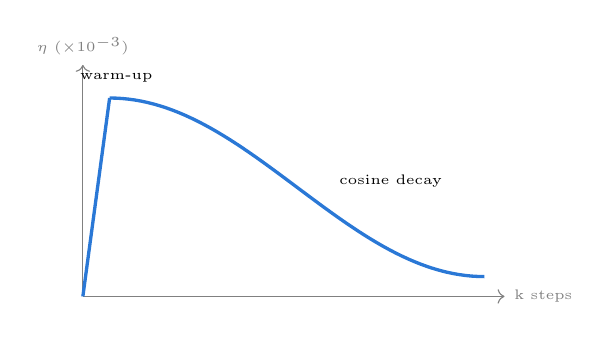
\begin{tikzpicture}[xscale=1.7,yscale=4.2]
        \draw[->,gray] (0,0)--(3.15,0) node[right,font=\tiny]{k steps};
        \draw[->,gray] (0,0)--(0,0.7) node[above,font=\tiny]{$\eta$ ($\times10^{-3}$)};
        \draw[very thick,accent] (0,0)--(0.2,0.6);
        \draw[very thick,accent,domain=0.2:3,samples=60] plot (\x,{0.06+0.27*(1+cos(180*(\x-0.2)/2.8))});
        \node[font=\tiny] at (0.25,0.66) {warm-up};
        \node[font=\tiny] at (2.3,0.35) {cosine decay};
      \end{tikzpicture}
      \begin{exampleblock}{Example}
        \small
        Peak $6\times10^{-4}$, 200 warm-up steps, 3,000 total. At step 100: $3\times10^{-4}$. At step 1,600, halfway through the decay: $3.3\times10^{-4}$. At step 3,000: $6\times10^{-5}$.
      \end{exampleblock}
    \end{column}
  \end{columns}
\end{frame}

\begin{frame}{Batches, steps and gradient accumulation}
  \twoterms{Batch, micro-batch, step and epoch}
  {A \textbf{batch} is the examples used for one weight update (a \textbf{step}). A \textbf{micro-batch} is what fits in GPU memory at once. An \textbf{epoch} is one full pass over the data.}
  {8 blocks of 1,024 tokens form one micro-batch. With 200M training tokens and 65,536 tokens per step, one epoch is about 3,050 steps.}
  {Gradient accumulation}
  {Run several micro-batches, adding up their gradients, before a single update. It gives a big effective batch on a small GPU.}
  {A T4 holds only 8 blocks at once. After 8 micro-batches, the effective batch is $8\times8\times1{,}024=65{,}536$ tokens. It is like filling a large tank with a small bucket: 8 trips, one pour.}
\end{frame}

\begin{frame}{Gradient clipping and exploding gradients}
  \term{Gradient clipping and gradient norm}
  {The \textbf{gradient norm} is the overall length of the gradient vector. If it exceeds a limit $c$, scale the whole gradient down to length $c$. The direction is kept, but the step is capped.}
  {A rare garbled OCR passage produces a gradient of norm 5.0. With $c=1.0$, every component is multiplied by $1/5=0.2$. One strange batch then cannot throw away hours of training. A log that shows norms constantly far above 1 is a warning sign.}
\end{frame}

\begin{frame}{Numerical precision}
  \twoterms{fp32, fp16 and bf16}
  {Floating-point formats. \textbf{fp32}: 32 bits, precise. \textbf{fp16}: 16 bits, fast, but the largest value is only 65,504 and tiny values round to zero. \textbf{bf16}: 16 bits with the \emph{same range} as fp32, but less precision.}
  {A gradient of $10^{-8}$ becomes 0 in fp16 (underflow), but survives in bf16. An attention score of 70,000 overflows fp16 to infinity. A T4 GPU supports fp16 but not bf16; an A100 supports both.}
  {Mixed precision and loss scaling (GradScaler)}
  {Do most maths in 16 bits for speed and keep sensitive parts, such as the loss and the weights, in fp32. For fp16, multiply the loss by a large factor before the backward pass so small gradients do not underflow, then divide it back out.}
  {Scale the loss by 1,024: a gradient of $10^{-8}$ becomes $10^{-5}$, which fp16 can hold. If an overflow appears, the scaler skips that step and halves the factor.}
\end{frame}

\begin{frame}{Checkpoints, resume and early stopping}
  \twoterms{Checkpoint (best vs last) and resume}
  {A saved snapshot of the weights, plus optimizer state for resuming. \textbf{best.pt} has the lowest validation loss so far. \textbf{last.pt} is the most recent. \textbf{Resume} continues from last.pt after an interruption.}
  {Colab disconnects at step 2,140. Rerunning the same command loads last.pt, saved at step 2,000, and loses only 140 steps. It is written \emph{atomically}, to a temporary file that is then renamed, so a crash mid-save never corrupts it.}
  {Early stopping and patience}
  {Stop training when validation loss has not improved for a set number of evaluations (the \textbf{patience}).}
  {Validation losses are 2.81, 2.79, 2.80, 2.82, 2.83. With patience 3, training stops after the last one and keeps the 2.79 checkpoint.}
\end{frame}

\begin{frame}{Throughput, memory and reproducibility}
  \twoterms{Throughput (tokens/s) and peak memory}
  {\textbf{Throughput} is tokens processed per second. \textbf{Peak GPU memory} is the most memory used at any moment. Together they decide what fits in a free Colab session.}
  {At 40,000 tokens/s, 200M tokens take $200\text{M}/40\text{k}=5{,}000$ s, about 1.4 hours. At 15,000 tokens/s it is 3.7 hours, which may need two sessions and a resume.}
  {Random seed and torch.compile}
  {A \textbf{seed} fixes the random number generators, so a run can be repeated exactly. \textbf{torch.compile} fuses operations into faster GPU kernels.}
  {Seed 1337 makes step 500 always draw the same blocks, even after a resume. That lets two learning rates be compared on identical data. torch.compile might raise throughput by 20--40\% on recent GPUs.}
\end{frame}

\begin{frame}{Compute environment}
  \twoterms{GPU, T4 and CUDA}
  {A \textbf{GPU} runs thousands of arithmetic operations in parallel. \textbf{CUDA} is NVIDIA's platform for programming it. The \textbf{T4} (16 GB) is the free Colab and Kaggle GPU.}
  {Multiplying two $768\times768$ matrices takes about 0.9 billion operations. A CPU does it in milliseconds, but a GPU runs thousands at once. MPS is Apple's equivalent on a Mac, used for our smoke test.}
  {Colab and Kaggle sessions}
  {Free hosted notebooks with a GPU for a limited time. Sessions can end without warning.}
  {Save runs to Google Drive by setting \code{paths.runs\_dir}. Otherwise a disconnect deletes the local disk, with every checkpoint on it.}
\end{frame}

% =====================================================================
\section{Decoding}

\begin{frame}{Greedy decoding and sampling}
  \twoterms{Greedy decoding}
  {Always pick the single most likely token ($\tau=0$). It is deterministic, but often repetitive.}
  {With $p$ = dismissed 0.45, allowed 0.30, disposed 0.15, greedy always writes ``dismissed''. It can loop: ``the court held that the court held that the court held\ldots''.}
  {Sampling}
  {Draw the next token at random from the probability distribution. Varied, and more human-like, but it can wander.}
  {It writes ``dismissed'' 45\% of the time, ``allowed'' 30\% and ``disposed'' 15\%. Occasionally it picks something odd from the long tail. That is why top-$k$ and top-$p$ exist.}
\end{frame}

\begin{frame}{Temperature}
  \begin{columns}[T]
    \begin{column}{0.5\textwidth}
      \term{Temperature $\tau$}
      {Divide the logits by $\tau$ before the softmax. $\tau<1$ sharpens the distribution (safer), $\tau>1$ flattens it (more creative), and $\tau\to0$ becomes greedy.}
      {Logits $[2,1,0]$ with $\tau=1$ give $[0.665,0.245,0.090]$. With $\tau=0.5$, they become $[4,2,0]$ and $p=[0.867,0.117,0.016]$. With $\tau=2$, they become $[1,0.5,0]$ and $p=[0.506,0.307,0.186]$.}
    \end{column}
    \begin{column}{0.46\textwidth}
      \centering
      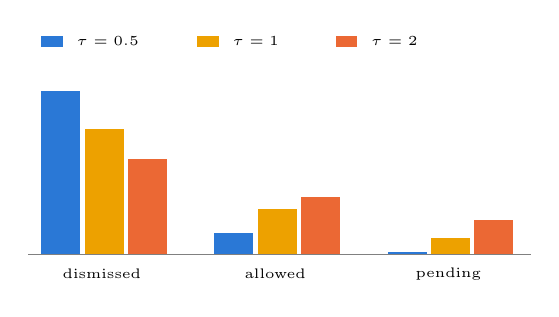
\begin{tikzpicture}[yscale=2.4,xscale=0.55]
        \foreach \x/\a/\b/\c in {0/0.867/0.665/0.506, 1/0.117/0.245/0.307, 2/0.016/0.090/0.186}{
          \fill[accent] (\x*4,0) rectangle ++(0.9,\a);
          \fill[gold] (\x*4+1,0) rectangle ++(0.9,\b);
          \fill[warm] (\x*4+2,0) rectangle ++(0.9,\c);}
        \draw[gray] (-0.3,0)--(11.3,0);
        \node[font=\tiny] at (1.4,-0.1) {dismissed};
        \node[font=\tiny] at (5.4,-0.1) {allowed};
        \node[font=\tiny] at (9.4,-0.1) {pending};
        \fill[accent] (0,1.1) rectangle ++(0.5,0.06); \node[font=\tiny,anchor=west] at (0.6,1.13) {$\tau=0.5$};
        \fill[gold] (3.6,1.1) rectangle ++(0.5,0.06); \node[font=\tiny,anchor=west] at (4.2,1.13) {$\tau=1$};
        \fill[warm] (6.8,1.1) rectangle ++(0.5,0.06); \node[font=\tiny,anchor=west] at (7.4,1.13) {$\tau=2$};
      \end{tikzpicture}
      \vspace{1mm}

      {\small Lower temperature puts more of the probability on the top choice.}
    \end{column}
  \end{columns}
\end{frame}

\begin{frame}{Top-$k$ and top-$p$ (nucleus) sampling}
  \begin{columns}[T]
    \begin{column}{0.485\textwidth}
      \term{Top-$k$}
      {Keep only the $k$ most likely tokens, renormalise, and sample among them. The long tail of nonsense is cut off.}
      {Probabilities $[0.50,0.20,0.15,0.10,0.05]$ with $k=2$ keep the first two. Renormalised, that is $[0.71,0.29]$. The rule is fixed: it keeps 2 tokens whether the model is confident or unsure.}
    \end{column}
    \begin{column}{0.485\textwidth}
      \term{Top-$p$ (nucleus)}
      {Keep the smallest set of top tokens whose total probability reaches $p$. The set size adapts to the model's confidence.}
      {Same probabilities with $p=0.9$: $0.50+0.20+0.15=0.85<0.9$, so add the next token, giving $0.95$. Four tokens are kept. For a confident step like $[0.93,0.04,\ldots]$, only one token is kept.}
    \end{column}
  \end{columns}
\end{frame}

\begin{frame}{Repetition control and length control}
  \twoterms{Repetition penalty and window}
  {Make tokens used recently less likely: divide positive logits by $r$, multiply negative ones by $r$. The \textbf{window} is how many recent tokens count.}
  {With $r=1.1$, ``court'' was just used and has logit $2.0$, which becomes $1.82$; a logit of $-1.0$ becomes $-1.1$. Too high a penalty stops the model repeating legitimate words such as ``appellant'', which legal text needs.}
  {Degeneration, EOS banning and the 128-word stop}
  {\textbf{Degeneration} is dull, looping or incoherent output. We \textbf{ban end-of-text} so the model never stops early, and stop once 129 complete words exist, keeping 128.}
  {If generation stopped at exactly 128 words, the last one could be half a token, like ``respond''. Waiting for the 129th guarantees word 128 is whole: ``respondent''.}
\end{frame}

\begin{frame}{Beam search (for later phases)}
  \term{Beam search}
  {Keep the $B$ best partial sequences at each step, extend each, and keep the $B$ best overall. It finds high-probability text, but can be bland. It is not used in our Phase-1 code, but is common for summarisation in Phase 6.}
  {With $B=2$, after ``The appeal'' the model keeps ``is'' (0.6) and ``stands'' (0.2). It expands both, and keeps the top two complete paths: ``is dismissed'' ($0.6\times0.5=0.30$) and ``is allowed'' ($0.6\times0.3=0.18$). The path through ``stands'' is dropped.}
\end{frame}

% =====================================================================
\section{Knowledge distillation}

\begin{frame}{Teacher, student and soft targets}
  \twoterms{Teacher and student}
  {A large trained \textbf{teacher} guides the training of a smaller \textbf{student}, so the student learns faster and better than from the data alone.}
  {The A1 teacher (82M parameters) trains an A4 student (47M). It is like a senior advocate coaching a junior, explaining how confident to be, not just what the right answer is.}
  {Soft targets and ``dark knowledge''}
  {The teacher's full probability distribution, not just the one correct token. It shows which wrong answers are nearly right.}
  {The true next word is ``dismissed''. The teacher says dismissed 0.6, rejected 0.3, allowed 0.1. The student learns that ``rejected'' is a near-synonym, information a one-hot label (1, 0, 0) never gives.}
\end{frame}

\begin{frame}{The distillation loss}
  \begin{columns}[T]
    \begin{column}{0.5\textwidth}
      \small
      \[
        \mathcal{L}=\alpha\,\mathcal{L}_{\text{CE}}+(1-\alpha)\,\tau^2\,\mathrm{KL}\big(p^T_\tau\,\|\,p^S_\tau\big)
      \]
      \begin{itemize}
        \item \textbf{KL divergence}: $\sum_i p_i\ln\frac{p_i}{q_i}$ measures how different two distributions are. It is 0 when they are identical.
        \item \textbf{Distillation temperature $\tau$}: softens both distributions, so small probabilities matter more.
        \item The $\tau^2$ factor keeps gradients comparable in size.
        \item $\alpha$ balances real labels against teacher guidance. We use 0.5.
      \end{itemize}
    \end{column}
    \begin{column}{0.46\textwidth}
      \begin{exampleblock}{Worked KL example}
        \small
        Teacher $p=[0.7,0.2,0.1]$ and student $q=[0.4,0.4,0.2]$:
        \[
          0.7\ln\tfrac{0.7}{0.4}+0.2\ln\tfrac{0.2}{0.4}+0.1\ln\tfrac{0.1}{0.2}
        \]
        \[
          =0.392-0.139-0.069=0.184
        \]
        Training pushes this toward 0: the student learns to put about 70\% on the teacher's favourite.
      \end{exampleblock}
    \end{column}
  \end{columns}
\end{frame}

\begin{frame}{Model compression}
  \term{Model compression}
  {Making a model smaller or faster while keeping most of its quality. Options include distillation, pruning (removing weights), quantisation (fewer bits per weight), and efficient architectures.}
  {The teacher has 82M parameters and a validation loss of 2.60. A distilled 47M student reaches 2.72; the same student trained without a teacher reaches 2.80. The student keeps most of the quality at 57\% of the size, and generates faster. (These numbers are illustrative, not measured.)}
\end{frame}

% =====================================================================
\section{Experiments and code engineering}

\begin{frame}{Designing experiments}
  \twoterms{Controlled experiment and ablation}
  {Change \textbf{one} factor, hold everything else fixed, and measure the effect. An \textbf{ablation} removes one component to see how much it mattered.}
  {Train A1 twice, identical except that the second run drops the Acts source. If validation loss on judgments barely moves but loss on statutes rises, Acts mainly help statute-style text.}
  {Baseline and hyperparameters}
  {A \textbf{baseline} is the simple reference system every idea is compared against. \textbf{Hyperparameters} are settings chosen by you, not learned, such as learning rate, layers or temperature.}
  {A1 is our baseline. ``A4 is better'' only means something as ``A4 reaches 0.05 lower loss than A1 on the same data and budget''. Note: 12 heads versus 16 heads is a hyperparameter change, not a new architecture.}
\end{frame}

\begin{frame}{Configuration system}
  \twoterms{YAML config and inheritance}
  {YAML is a readable text format for settings. \textbf{Inheritance} (\code{inherit: base.yaml}) lets one file extend another and override only what differs.}
  {\code{a4\_efficient.yaml} is only 14 lines. It inherits all the data, tokenizer and training settings from \code{base.yaml} and adds its own model shape. Changing the token budget in base.yaml changes it for all four models at once.}
  {Command-line overrides}
  {\code{--set key.sub=value} changes one setting for one run, without editing any file.}
  {\code{--set train.lr=3e-4 run\_name=A1\_lr3e-4} makes a new run folder whose saved \code{config.yaml} records exactly what changed. That record is evidence for the report.}
\end{frame}

\begin{frame}{Testing}
  \twoterms{Smoke test}
  {A quick end-to-end run on tiny data, to check the whole pipeline works before spending hours of GPU time.}
  {\code{run\_smoke\_test.sh} builds a fake legal corpus and trains all four models for 40 steps. It then generates, scores and zips the predictions, in a few minutes on a laptop. A broken zip layout is caught here, not on Codabench.}
  {Unit tests: causality and cache correctness}
  {Small automatic checks of one property each. \textbf{Causality}: changing a future token must not change past predictions. \textbf{Cache correctness}: cached generation must equal a full recomputation.}
  {If a mask bug let position 10 see position 40, the causality test fails at once. Without the test, the model would ``cheat'' in training, then fall apart at generation time.}
\end{frame}

% =====================================================================
\section{Index}

\begin{frame}{Alphabetical index (A--C)}
  \footnotesize
  \begin{multicols}{3}
  \begin{itemize}\setlength{\itemsep}{0pt}
    \item Ablation -- Experiments
    \item Activation functions -- Blocks
    \item AdaLoRA -- LoRA family
    \item AdamW -- Training
    \item Adapters (Houlsby, Pfeiffer) -- Project
    \item ALiBi -- Architectures
    \item Attention mask -- Blocks
    \item Autoregressive LM -- LM basics
    \item Baseline -- Experiments
    \item Batch, micro-batch -- Training
    \item Beam search -- Decoding
    \item BERTScore -- Metrics
    \item bf16, fp16, fp32 -- Training
    \item Big-O, FLOPs -- Architectures
    \item BitFit -- Project
    \item Bits per word -- Metrics
    \item BLEU-4, brevity penalty -- Metrics
    \item BPE, byte-level BPE -- Tokenization
    \item Budget schedule -- LoRA family
    \item Calibration -- Project
    \item Causal mask -- Blocks
    \item Checkpoint (best, last) -- Training
    \item Chunking -- Project
    \item Class imbalance -- Metrics
    \item Codabench -- Project
    \item Contextual embedding -- Metrics
    \item Context window -- LM basics
    \item Continuation loss -- LM basics
    \item Contrastive learning -- Project
    \item Corpus -- Data
    \item Cosine decay -- Training
    \item Cosine similarity -- Metrics
    \item Cross-attention -- Architectures
    \item Cross-entropy -- LM basics
    \item CUDA, GPU, T4 -- Training
  \end{itemize}
  \end{multicols}
\end{frame}

\begin{frame}{Alphabetical index (D--H)}
  \footnotesize
  \begin{multicols}{3}
  \begin{itemize}\setlength{\itemsep}{0pt}
    \item Data leakage -- Data
    \item Data mixing -- Data
    \item Decoder, decoder-only -- Architectures
    \item Degeneration -- Decoding
    \item Dev set -- Data
    \item Distillation -- Distillation
    \item Document-level split -- Data
    \item Double quantisation -- LoRA family
    \item Dropout -- Blocks
    \item Early stopping -- Training
    \item Embedding (token, tied) -- Blocks
    \item Encoder, encoder--decoder -- Architectures
    \item End-of-text token -- Data
    \item Epoch -- Training
    \item Extractive, abstractive -- Project
    \item Extrapolation -- Architectures
    \item Fertility -- Tokenization
    \item Fine-tuning -- Project
    \item Foundation model -- Project
    \item From scratch -- LM basics
    \item Gated dataset -- Project
    \item GELU, ReLU, SiLU -- Blocks
    \item GPT-2 tokenizer -- Tokenization
    \item Gradient accumulation -- Training
    \item Gradient clipping, norm -- Training
    \item Gradient descent -- Training
    \item GradScaler, loss scaling -- Training
    \item Greedy decoding -- Decoding
    \item Grouped-query attention -- Architectures
    \item Hard negative -- Project
    \item Hierarchical model -- Project
    \item Hyperparameter -- Experiments
  \end{itemize}
  \end{multicols}
\end{frame}

\begin{frame}{Alphabetical index (I--M)}
  \footnotesize
  \begin{multicols}{3}
  \begin{itemize}\setlength{\itemsep}{0pt}
    \item IA$^3$ -- Project
    \item Importance score (sensitivity) -- LoRA family
    \item Initialisation -- Blocks
    \item Intrinsic rank -- LoRA family
    \item JSON, JSON Lines -- Data
    \item KL divergence -- Distillation
    \item KV-cache -- Architectures
    \item Language model -- LM basics
    \item Layer freezing -- Project
    \item LayerNorm, pre-LN -- Blocks
    \item Learned positions -- Architectures
    \item Learning rate, warm-up -- Training
    \item Left-truncation -- Architectures
    \item Logits -- LM basics
    \item LoRA -- LoRA family
    \item LORMA -- LoRA family
    \item Macro-F1, Micro-F1 -- Metrics
    \item Memory map -- Data
    \item Merging adapters -- LoRA family
    \item Micro-F1@7 -- Metrics
    \item Mixed precision -- Training
    \item Model compression -- Distillation
    \item Momentum -- Training
    \item Multi-head attention -- Blocks
    \item Multi-label -- Project
    \item Multi-query attention -- Architectures
  \end{itemize}
  \end{multicols}
\end{frame}

\begin{frame}{Alphabetical index (N--R)}
  \footnotesize
  \begin{multicols}{3}
  \begin{itemize}\setlength{\itemsep}{0pt}
    \item NER, strict span match -- Project
    \item NF4 (NormalFloat) -- LoRA family
    \item Orthogonality regulariser -- LoRA family
    \item Overfitting, underfitting -- Training
    \item Padded vocabulary -- Architectures
    \item Padding -- Architectures
    \item Paged optimizer -- LoRA family
    \item Parameters -- LM basics
    \item PEFT -- Project
    \item Perplexity -- LM basics
    \item Pooling -- Project
    \item Precision, recall, F1 -- Metrics
    \item Prediction.json -- Project
    \item Prefill, decode -- Architectures
    \item Prefix-LM -- Architectures
    \item Prefix -- LM basics
    \item Prefix tuning -- Project
    \item Pre-training -- Project
    \item Prior case retrieval -- Project
    \item Prompt tuning -- Project
    \item QLoRA -- LoRA family
    \item Query, key, value -- Blocks
    \item Rank inflation -- LoRA family
    \item Rank, low-rank matrix -- LoRA family
    \item Regularisation -- Training
    \item Repetition penalty -- Decoding
    \item Residual connection -- Blocks
    \item Resume -- Training
    \item Rhetorical roles -- Project
    \item RMSNorm -- Blocks
    \item Rolling cache -- Architectures
    \item RoPE -- Architectures
    \item ROUGE-L, LCS -- Metrics
    \item rsLoRA -- LoRA family
  \end{itemize}
  \end{multicols}
\end{frame}

\begin{frame}{Alphabetical index (S--Z)}
  \footnotesize
  \begin{multicols}{3}
  \begin{itemize}\setlength{\itemsep}{0pt}
    \item Sampling -- Decoding
    \item Scaling factor $\alpha/r$ -- LoRA family
    \item Seed -- Training
    \item Self-attention -- Blocks
    \item Self-hosted model -- Project
    \item Sinusoidal positions -- Architectures
    \item Sliding window -- Architectures
    \item Smoke test -- Experiments
    \item Softmax -- LM basics
    \item Soft targets -- Distillation
    \item Special tokens -- Tokenization
    \item Streaming -- Data
    \item Subset accuracy -- Metrics
    \item SVD -- LoRA family
    \item SwiGLU -- Blocks
    \item Teacher, student -- Distillation
    \item Temperature -- Decoding
    \item Threshold -- Project
    \item Throughput -- Training
    \item Token bin, uint16 -- Data
    \item Tokenizer -- Tokenization
    \item Token, token budget -- Data
    \item Top-$k$, top-$p$ -- Decoding
    \item torch.compile -- Training
    \item Train, val, dev, test -- Project
    \item Unit test -- Experiments
    \item Unknown token, OOV -- Tokenization
    \item Vocabulary -- Tokenization
    \item Weight decay -- Training
    \item YAML, inheritance -- Experiments
  \end{itemize}
  \end{multicols}
\end{frame}

\end{document}
